% Created 2019-11-09 Sat 17:57
% Intended LaTeX compiler: pdflatex
\documentclass{scrartcl}
\usepackage[utf8]{inputenc}
\usepackage[T1]{fontenc}
\usepackage{graphicx}
\usepackage{grffile}
\usepackage{longtable}
\usepackage{wrapfig}
\usepackage{rotating}
\usepackage[normalem]{ulem}
\usepackage{amsmath}
\usepackage{textcomp}
\usepackage{amssymb}
\usepackage{capt-of}
\usepackage{hyperref}
\hypersetup{colorlinks,linkcolor=black,urlcolor=blue}
\usepackage{textpos}
\usepackage{textgreek}
\usepackage[version=4]{mhchem}
\usepackage{chemfig}
\usepackage{siunitx}
\usepackage{gensymb}
\usepackage[usenames,dvipsnames]{xcolor}
\usepackage[T1]{fontenc}
\usepackage{lmodern}
\usepackage{verbatim}
\usepackage{tikz}
\usepackage{wasysym}
\usetikzlibrary{shapes.geometric,arrows,decorations.pathmorphing,backgrounds,positioning,fit,petri}
\usepackage{fancyhdr}
\pagestyle{fancy}
\author{Matthew Henderson, PhD, FCACB}
\date{\today}
\title{Organelle Related Disorders}
\hypersetup{
 pdfauthor={Matthew Henderson, PhD, FCACB},
 pdftitle={Organelle Related Disorders},
 pdfkeywords={},
 pdfsubject={},
 pdfcreator={Emacs 26.1 (Org mode 9.1.9)}, 
 pdflang={English}}
\begin{document}

\maketitle
\tableofcontents


\section{Sphingolipid Synthesis}
\label{sec:org4aaf625}
\subsection{Introduction}
\label{sec:orgc02aedd}
\begin{enumerate}
\item Sphingolipids
\label{sec:org5fb80ad}
\begin{itemize}
\item Found in all mammalian cell membranes
\item Plasma lipoproteins
\item Structural role
\item Modulate numerous biological functions
\begin{itemize}
\item apoptosis
\end{itemize}
\item named after the Sphinx because of their enigmatic nature
\end{itemize}

\item Sphingosine and Ceramide
\label{sec:org03a20a2}

\begin{itemize}
\item long chain sphingolipid base
\item N-acylated by a variety of fatty acids
\end{itemize}

\definesubmol{x}{-[7,.3]-[1,.3]}
\definesubmol{y}{-[:+30,.3]=[:-30,.3]}
\definesubmol{a}{-[1,.3](=[2,.3]O)!x!x!x!x!x!x!x!x!x!x!x}
\chemname{\chemfig{OH!x([2,.5]<HN)-[7,.3](-[6,.3]OH)-[1,.3]=[7,.3]-[1,.3]!x!x!x!x!x!x}}{sphingosine}
\chemname{\chemfig{OH!x([2,.5]<HN!a)-[7,.3](-[6,.3]OH)-[1,.3]=[7,.3]-[1,.3]!x!x!x!x!x!x}}{sphingolipid}
%%\chemfig{!b}

\item Biosynthesis
\label{sec:org3d653d5}

\begin{enumerate}
\item ER
\label{sec:org03b3856}
\begin{itemize}
\item condensation of serine and palmitoyl-CoA \(\to\) sphinganine
\item N-acylation \(\to\) ceramide
\end{itemize}

\item Golgi
\label{sec:org8726464}
\begin{itemize}
\item stepwise addition of monosaccharides
\begin{itemize}
\item sphingomyelin
\item glucosylceramide
\item glycosphingolipids
\item gangliosides
\end{itemize}
\end{itemize}


\begin{figure}[htbp]
\centering
\includegraphics[width=\textwidth]{./sphingolipid_synthesis/figures/Sphingolipids_general_structures.png}
\caption[Sphingolipid Structure]{\label{fig:orgeaaa2d6}
Sphingolipid Structure}
\end{figure}


\begin{figure}[htbp]
\centering
\includegraphics[width=0.8\textwidth]{./sphingolipid_synthesis/figures/synthesis.png}
\caption[Sphingolipid Biosynthesis]{\label{fig:org01b85fa}
Sphingolipid Biosynthesis}
\end{figure}
\end{enumerate}
\end{enumerate}

\subsection{Disorders of Sphingolipid Synthesis}
\label{sec:org8035af3}
\begin{enumerate}
\item Classification
\label{sec:orgaac6e1d}

\begin{enumerate}
\item Primarily nervous system involvement
\label{sec:org0e13394}
\begin{itemize}
\item Serine palmitoyltransferase - peripheral sensory neuropathy
\item Ceramide synthase 1 - myoclonic epilepsy
\item Ceramide synthase 2 - myoclonic epilepsy
\item Fatty Acid 2-hydroxylase - SPG35
\item Nonlysosomal β-Glucosidase - SPG46
\item GM3 Synthase Deficiency - Amish infantile epilepsy
\item GM2/GD2 Synthase Deficiency - SPG26
\end{itemize}

\item Primarily skin involvement
\label{sec:orge2e82ef}
\begin{itemize}
\item Ceramide synthase 3 - Ichthyosis
\item ULCFA \(\omega\)-hydrolase - Ichthyosis
\end{itemize}
\end{enumerate}


\item Serine Palmitoyltransferase (Subunit 1 or 2) Deficiency
\label{sec:org6dcfc7f}

\begin{itemize}
\item Defect in first step of sphingolipid biosynthesis
\item Major cause of dominant Hereditary Sensory and Autonomic Neuropathies (HSAN1).
\begin{itemize}
\item Late onset (2-4th decade)
\item peripheral sensory neuropathy
\item distal sensory loss
\item ulcerative mutilations
\item hypohydrosis
\item there is a more severe early onset form
\end{itemize}
\item Accumulation of sphingoid bases \(\to\) pathology
\item mutations in serine palmitoyltransferase (SPCTLC1 or 2) alter
substrate specificity
\begin{itemize}
\item serine \(\to\) alanine and glycine
\end{itemize}
\item Elevated plasma 1-deoxy-sphingamine, 1-deoxy-methyl-sphingamine, 1-deoxy-ceramindes
\item Trial of serine supplementation
\end{itemize}

\item Ceramide Synthases 1 and 2
\label{sec:org9beecc2}

\begin{itemize}
\item Six human ceramide synthases
\begin{itemize}
\item tissue and acyl-CoA substrate specificity
\item Neurological CERS1 \&2
\begin{description}
\item[{CER1}] Myoclonic epilepsy, cognitive decline
\begin{itemize}
\item Decreased C18-ceramide in cultured fibroblasts
\end{itemize}
\item[{CER2}] Myoclonic epilepsy
\begin{itemize}
\item Decreased VLC-ceramide in cultured fibroblasts
\end{itemize}
\end{description}
\item Dermatologic CERS3
\begin{description}
\item[{CER3}] Ichthyosis
\begin{itemize}
\item Lack of VLC-ceramides in skin and fibroblasts
\end{itemize}
\end{description}
\end{itemize}
\end{itemize}

\item Fatty Acid 2-Hydroxylase
\label{sec:orgef46549}

\begin{itemize}
\item spastic paraplegia
\begin{itemize}
\item fatty acid hydroxylase associated neurodegeneration (FAHN)
\end{itemize}
\item 38 patients, most in present in childhood
\item slowly progressing
\begin{itemize}
\item spastic paraplegia
\item dysarthria
\item mild cognitive decline
\item dystonia
\end{itemize}

\item Insufficiency production of 2-hydroxy-galactosphingolipids
\begin{itemize}
\item required in myelin
\item increase with brain development
\end{itemize}

\item Decreased hydroxylated sphingomyelin in cultured cells
\end{itemize}

\item GM3 Synthase Deficiency
\label{sec:org0d6ec20}

\begin{itemize}
\item Autosomal recessive infantile-onset epilepsy
\begin{itemize}
\item Amish epilepsy syndrome
\end{itemize}
\item In first year \(\to\) generalized tonic-clonic seizures
\begin{itemize}
\item profound developmental stagnation and regression
\item salt and pepper syndrome
\begin{itemize}
\item hyper and hypo-pigmented skin maculae
\item facial dysmorphism scoliosis
\item intellectual disability
\item seizures
\item choreoathetosis
\item spasticity
\end{itemize}
\end{itemize}

\item lack of GM3, GD3 and higher gangliosides, and increased
lactosylceramide and Gb4 levels in plasma and cultured cells
\end{itemize}

\item GM2/GD2 Synthase Deficiency
\label{sec:org8d9a441}

\begin{itemize}
\item Mutations of B4GALNT1
\item SPG26, a slowly progressive complex hereditary spastic paraplegia
with mild to moderate cognitive impairment.

\item Cultured fibroblasts of patients have shown decreased GM2 levels
with an increase of its precursor, GM3.
\end{itemize}

\item Non-lysosomal β-Glucosidase Deficiency
\label{sec:org9f7ba44}

\begin{itemize}
\item GBA2 is a membrane-associated protein localised at the ER and Golgi
\begin{itemize}
\item hydrolyse glucosylceramide to ceramide and glucose.
\end{itemize}
\item GBA2 is distinct from the lysosomal acid \(\beta\)-glucosidase GBA1 deficient in Gaucher disease
\item hereditary (complex) spastic paraplegia locus SPG46.
\item Starting in childhood marked spasticity in lower extremities with
progressive gait disturbances
\begin{itemize}
\item later, ataxia and other cerebellar signs
\end{itemize}
\end{itemize}

\item Ceramide Synthase 3 and ULFA \(\omega\)-Hydroxylase
\label{sec:orgb265656}

\begin{itemize}
\item ceramides in skin maintain skin barrier homeostasis, prevent water
loss and protect against microbial infections
\item Autosomal recessive congenital ichthyosis (ARCI) is a heterogeneous
group of disorders of epidermal cornification
\item 9 causative genes have been identified including CERS3 and CYP4F22

\item[{CERS3}] ichthyosis
\begin{itemize}
\item lack of ceramides with VLCFA in cultured fibroblasts
\end{itemize}
\item[{CYP4F22}] ichthyosis
\begin{itemize}
\item lack of ceramides with ULCFA in cultured fibroblasts
\end{itemize}
\end{itemize}
\end{enumerate}

\section{Sphingolipidoses}
\label{sec:org3963130}

\begin{table}[htbp]
\caption{\label{tab:orgf4b8735}
The Sphingolipidoses}
\centering
\begin{tabular}{llll}
Disease & Enzyme & Sphingolipid & Prevalence\\
\hline
Gaucher & \(\beta\)-glucocerebrosidase & glucocerebroside & 1:50,000\\
Fabry & \(\alpha\)-galactosidase A & globotriaosylceramide (Gb3) & 1:80,000\\
MLD & arylsulfatase A & sulfatide & 1:100,000\\
GM1 & \(\beta\)-gangliosidase & GM1 ganglioside & 1:200,000\\
Krabbe & galactocerebrosidase & galactosylceramide & 1:250,000\\
NPA/B & acid sphingmyelinase & sphingomyelin & 1:250,000\\
GM2 & HexA and/or HexB & GM2 ganglioside & 1:300,000 (HexA)\\
Farber & acid ceramidase & ceramides & 1:1,000,000\\
\end{tabular}
\end{table}

\begin{figure}[htbp]
\centering
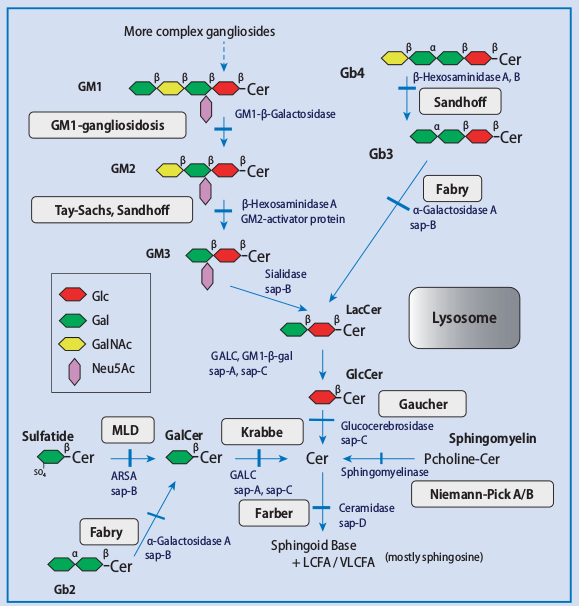
\includegraphics[width=0.8\textwidth]{./figures/sl_degradation.png}
\caption{\label{fig:org0dd5ea2}
Sphingolipid degradation}
\end{figure}

\subsection{Protein Trafficking to Lysosome}
\label{sec:org989c14b}
\begin{itemize}
\item Lysosomes are composed of soluble and transmembrane proteins that
are targeted to lysosomes in a signal-dependent manner.
\item The majority of soluble acid hydrolases are modified with mannose
6-phosphate (M6P) residues, allowing their recognition by M6P
receptors in the Golgi complex and ensuing transport to the
endosomal/lysosomal system.
\item Other soluble enzymes and non-enzymatic proteins are transported to
lysosomes in an M6P-independent manner mediated by alternative
receptors such as the lysosomal integral membrane protein LIMP-2 or
sortilin.
\item Sorting of cargo receptors and lysosomal transmembrane proteins
requires sorting signals present in their cytosolic domains.
\item These signals include dileucine-based motifs, DXXLL or [DE]XXXL[LI],
and tyrosine-based motifs, YXXØ, which interact with components of
clathrin coats such as GGAs or adaptor protein complexes.
\item In addition, phosphorylation and lipid modifications regulate signal
recognition and trafficking of lysosomal membrane proteins.
\end{itemize}

\begin{figure}[htbp]
\centering
\includegraphics[width=0.9\textwidth]{./figures/protein_trafficking.jpg}
\caption{\label{fig:orgc329044}
Protein Trafficking to Lysosome}
\end{figure}

\begin{figure}[htbp]
\centering
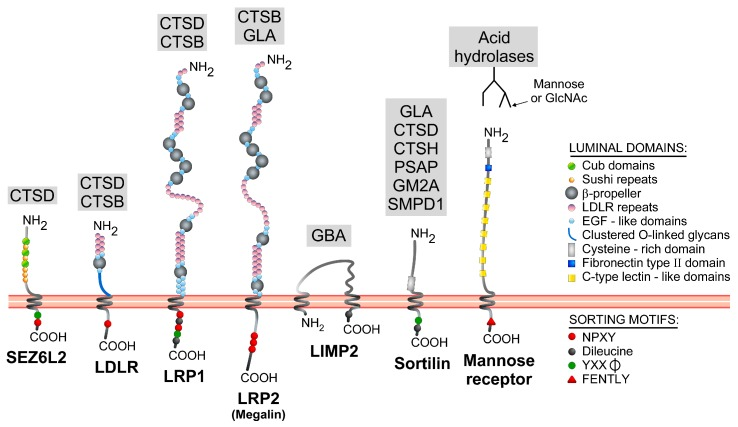
\includegraphics[width=0.8\textwidth]{./figures/lysosome_trafficking.jpeg}
\caption[Lysosomal protein trafficking receptors]{\label{fig:org41274f1}
Lysosomal protein trafficking receptors}
\end{figure}


\subsection{M6P receptors}
\label{sec:org5ee2783}
\begin{itemize}
\item MPRs are transmembrane glycoproteins that target enzymes to lysosomes in vertebrates
\item MPRs bind newly synthesized lysosomal hydrolases in the TGN and deliver them to pre-lysosomal compartments.
\item There are two different MPRs
\begin{itemize}
\item the cation-independent mannose 6-phosphate receptor (CI-MPR),
\item CD-MPR requires divalent cations to efficiently recognize lysosomal hydrolases
\end{itemize}
\end{itemize}
-bind terminal M6-P with similar affinity7

\subsection{Sortilin}
\label{sec:orgf189dbc}
\begin{itemize}
\item Sortilin is a type I transmembrane protein found in lysosomes
\begin{itemize}
\item can transport several lysosomal proteins from the TGN or PM to the endosomes
\end{itemize}
\item Tissues from sortilin knock-out mice exhibit normal morphology
\item Sortilin may transport selected acid hydrolases in:
\begin{itemize}
\item a subset of cell types
\item under stress conditions (e.g. Man-6-P pathway is deficient)
\end{itemize}
\end{itemize}

\subsection{LIMP2}
\label{sec:org45c994d}
\begin{itemize}
\item LIMP-2 in a membrane protein in lysosomes that functions to regulate lysosomal/endosomal transport.
\item type III glycoprotein that is located primarily in limiting membranes of lysosomes and endosomes.
\item may participate in membrane transportation and the reorganization of endosomal/lysosomal compartment.
\end{itemize}

\subsection{Megalin}
\label{sec:orgdd9306d}
\begin{itemize}
\item a cell surface receptor involved in reabsorption of proteins at the kidney proximal tubule
\item megalin mediated endocytosis of \(\alpha\)-galactosidase kidney proximal tubule
\item megalin also mediates the endocytosis of \(\alpha\)-galactosidase in renal podocytes
\end{itemize}

\subsection{Gaucher}
\label{sec:org2c56115}
\begin{enumerate}
\item Introduction
\label{sec:org128b886}
\begin{itemize}
\item Caused by accumulation of \textbf{glucosylceramide (glucocerebroside)}.
\begin{itemize}
\item - Glucocerebroside is the Gaucher lipid
\end{itemize}
\item Defect in \textbf{\(\beta\)-glucocerebrosidase}
\begin{itemize}
\item Extremely rare \textbf{SAP-C deficiency}
\end{itemize}
\item Most common LSD
\begin{itemize}
\item 1:40,000 to 1:50,000 live births
\end{itemize}
\item Three types:
\begin{description}
\item[{Type 1}] No neurological symptoms
\item[{Type 2}] Acute neuronopathic
\item[{Type 3}] Sub-acute or chronic neuronopathic
\end{description}
\item Type 1 disease is common in Western Europe, the Americas and Israel
\item In many other countries neuronopathic forms of Gaucher disease predominate
\end{itemize}


\begin{itemize}
\item Located in the lumen of lysosomes
\item LIMP-2 is responsible for mannose 6-phosphate receptor independent
lysosomal targeting of \(\beta\)-glucocerebrosidase
\end{itemize}

\begin{figure}[htbp]
\centering
\includegraphics[width=0.5\textwidth]{./gaucher/figures/glucocerebroside.png}
\caption{\label{fig:org1458b56}
Glucocerebroside the Gaucher Lipid}
\end{figure}

\begin{figure}[htbp]
\centering
\includegraphics[width=0.5\textwidth]{./gaucher/figures/glucocerebrosidase.png}
\caption{\label{fig:org907495e}
\(\beta\)-glucocerebrosidase defective in Gaucher}
\end{figure}

\item Genetics
\label{sec:org03b332a}
\begin{itemize}
\item Autosomal recessive, GBA gene
\item Most of the >300 disease alleles in Gaucher disease are missense
mutations
\begin{itemize}
\item result in \(\beta\)-glucocerebrosidase with decreased catalytic
function and/or stability.
\end{itemize}
\item A variety of complex mutations/rearrangements also causes Gaucher
disease:
\begin{itemize}
\item missense mutations, frame shift mutations, splicing mutations,
deletions, gene fusions with the pseudogene, examples of gene
conversions, and total deletions.
\end{itemize}
\item genotype/phenotype correlations exist for:
\begin{itemize}
\item type 1 disease (N370S)
\item types 2 and 3 (L444P)
\end{itemize}
\item within these categories there is variable penetrance and
expressivity between individuals and ethnic groups.
\end{itemize}

\item Clinical Findings
\label{sec:org16130a3}
\begin{table}[htbp]
\caption{\label{tab:orgabd4f83}
Gaucher Clinical Variants}
\centering
\begin{tabular}{llll}
 & Type 1 & Type 2 & Type 3\\
\hline
Onset & Infant/Child/Adult & 3-6 months & Childhood\\
Neurodegeneration & Absent & \texttt{++++} & \texttt{++} \(\to\) \texttt{++++}\\
Survival & 6 - 80+ years & < 2 years & 2nd - 4th decade\\
Splenomegaly & \texttt{++++} & \texttt{++} & \texttt{++}\\
Hepatomegaly & \texttt{++} & \texttt{++} & \texttt{+}\\
Fractures, bone crises & \texttt{+} & - & \texttt{+}\\
Enrichment & Ashkenazi & None & Norrbottnian\\
 &  &  & Swedish\\
\end{tabular}
\end{table}

\begin{enumerate}
\item Gaucher type 1
\label{sec:orgad53ca8}
\begin{itemize}
\item Clinical manifestations of Gaucher type 1 are linked to macrophages
engorged with glucosylceramide.

\item An undefined mechanism results in:
\begin{itemize}
\item enlargement and dysfunction of the liver and spleen
\item displacement of normal bone marrow by storage cells
\item osteoclastic-osteoblastic imbalances
\begin{itemize}
\item subsequent damage leading to bone infarctions and fractures.
\end{itemize}
\item Occasionally, involvement of other organs (e.g. lung) contributes
to the overall clinical picture.
\item Hypermetabolism and cachexia can be present
\item Thrombocytopenia is the most common peripheral blood abnormality
\end{itemize}

\item Neurological manifestations include:
\begin{itemize}
\item a high incidence of Parkinsonism
\item spinal cord compression
\item nerve root compression
\item polyneuropathy.
\end{itemize}
\end{itemize}

\item Gaucher type 2
\label{sec:org016cca6}
\begin{itemize}
\item Type 2 is the rarer of the two classic neuronopathic variants
\item early infantile onset of acute neuronopathic disease
\item progressing rapidly to death before age 2 years

\begin{itemize}
\item retroflexion of the neck
\item developmental delay, poor weight gain,
\item protuberant abdomen due to hepatosplenomegaly
\item Bulbar signs are prominent including:
\begin{itemize}
\item convergent squint, ocular paresis, trismus, dysphagia
\end{itemize}
\end{itemize}

\item The perinatal-lethal subtype is the most severe form of Gaucher
disease.
\begin{itemize}
\item leads to death in utero or within hours to days after
birth
\end{itemize}
\end{itemize}

\item Gaucher type 3
\label{sec:org589a011}
\begin{itemize}
\item type 3 disease has a later onset, with slower progression of
neurologic manifestations and variable degrees of systemic
involvement.
\item phenotype in type 3 Gaucher disease is considerably more
heterogeneous than that in type 2.

\item onset of symptoms occurs later, and neurologic involvement
progresses more slowly

\item includes abnormalities in:
\begin{itemize}
\item eye movements, seizures, intellectual deterioration
\end{itemize}

\item The same systemic manifestations occur as in type 1 disease.
\begin{itemize}
\item many type 3 patients may be incorrectly classified as type 1 when
first seen
\end{itemize}
\end{itemize}

\begin{enumerate}
\item Gaucher type 3a
\label{sec:orgedfdf6c}
\begin{itemize}
\item progressive myoclonus and dementia
\end{itemize}

\item Gaucher type 3b
\label{sec:org2b1ce6a}
\begin{itemize}
\item horizontal supranuclear gaze palsy without other major
neurologic signs
\item aggressive systemic disease
\end{itemize}

\item Gaucher type 3c
\label{sec:org5aefd72}
\begin{itemize}
\item present in late childhood or later
\item only mild visceral signs of classic Gaucher disease
\item distinguishing clinical signs include:
\begin{itemize}
\item impaired horizontal ocular saccades
\item corneal opacities
\item cardiac/aortic valvular calcification
\end{itemize}
\end{itemize}
\end{enumerate}
\end{enumerate}

\item Laboratory Investigations
\label{sec:org0411898}
\begin{figure}[htbp]
\centering
\includegraphics[width=0.6\textwidth]{./gaucher/figures/Gaucher_Cells_with_Fibrillar_Appearing_Cytoplasm.jpg}
\caption{\label{fig:orge2fbe95}
Gaucher Cells}
\end{figure}

\begin{enumerate}
\item Biochemistry
\label{sec:org892e3e4}
\begin{enumerate}
\item Enzyme Assay
\label{sec:orgba8cd5f}
\begin{itemize}
\item assay of the \(\beta\)-glucocerebrosidase activity in any nucleated cell
\begin{itemize}
\item the enzyme does not normally occur in plasma/serum or erythrocytes
\end{itemize}
\item Glucocerebrosidase activity in:
\begin{itemize}
\item peripheral blood lymphocytes/leukocytes
\item dried blood spots
\end{itemize}
\item 4MU-\(\beta\)-D--glucopyranoside substrate
\end{itemize}

\item Monitoring
\label{sec:org9038fad}
\begin{itemize}
\item chitotriosidase, chemokine CLL18/PARK, glucosylsphingosine
\end{itemize}
\end{enumerate}

\item Molecular
\label{sec:org0c41845}
\begin{itemize}
\item GBA gene sequencing, >300 disease alleles
\item Patients homozygous for the L444P mutation have severe visceral
disease, highly predisposed to the development of CNS disease.
\item The N370S mutant enzyme appears to preclude the development of classical CNS disease of Gaucher disease.
\item The D409H mutation manifests a characteristic phenotype:
\begin{itemize}
\item including cardiac calcification, oculomotor apraxia, and corneal opacities.
\end{itemize}
\end{itemize}
\end{enumerate}

\item Treatment
\label{sec:org16d7aad}
\begin{enumerate}
\item Bone marrow transplantation
\label{sec:org068aa94}
\begin{itemize}
\item Curative for Type 1
\begin{itemize}
\item Suggests hematopoietic gene therapy
\end{itemize}
\item High risk of mortality
\end{itemize}
\item ERT
\label{sec:org9b36f72}
\begin{itemize}
\item treats: hematological, visceral, and bony disease
\begin{itemize}
\item not cerebral disease
\end{itemize}
\item macrophages have a mannose receptor
\begin{itemize}
\item glucocerebrosidase glycoprotein modified to expose terminal mannose
\end{itemize}
\item 1991, Ceredase (algucerase) - human placenta
\item 1994, Cerezyme (imiglucerase) - CHO cells
\item 2010, VPRIV (velaglucerase) - human fibroblasts
\end{itemize}

\item Substrate reduction therapy
\label{sec:org8b227f8}
\begin{itemize}
\item ceramide glucoyltransferase inhibitor
\begin{itemize}
\item N-butyldeoxynojirimycin (miglustate)
\item eliglustat tartrate
\end{itemize}
\item Chaperone to stabilize - missense mutation
\begin{itemize}
\item isofagomine
\end{itemize}
\end{itemize}
\end{enumerate}
\end{enumerate}

\subsection{Niemann-Pick  A \& B}
\label{sec:org434eb4b}
\begin{enumerate}
\item Introduction
\label{sec:orgcd965d5}
\begin{itemize}
\item There are two distinct diseases called Niemann-Pick
\begin{itemize}
\item Types A and B (acid sphingomyelinase deficiency)
\item Type C (cholesterol recycling) - see section \ref{sec:orgb796ab7}
\end{itemize}

\item Incidence of Niemann-Pick A among Ashkenazi Jews \textasciitilde{} 1:40,000.
\item Incidence of both Niemann-Pick A and B in all other populations \textasciitilde{} 1:250,000.
\item Niemann-Pick Type A and B are caused by deficiency of \textbf{acid sphingomyelinase (ASM)}
\begin{itemize}
\item acid sphingomyelinase is required to metabolize sphingomyelin.
\item results in progressive \textbf{accumulation of sphingomyelin} in systemic organs
\begin{itemize}
\item brain accumulation in neuronal forms
\end{itemize}
\item There is growing evidence that NPA \& NPB represent opposite ends of a continuum.
\begin{itemize}
\item NPA generally have little or no ASM production (less than 1\% of normal).
\item NPB have approximately 10\% of normal level of ASM.
\end{itemize}
\end{itemize}
\item lysosomal trafficking of acid sphingomyelinase is mediated by sortilin and mannose 6-phosphate receptor.
\item MPR alone is sufficient to transport NPC2 to the endo/lysosomal compartment
\end{itemize}


\begin{figure}[htbp]
\centering
\includegraphics[width=0.4\textwidth]{./niemann_pick/figures/sphingomyelin.png}
\caption{\label{fig:org0831c66}
Sphingomyelin}
\end{figure}

\begin{figure}[htbp]
\centering
\includegraphics[width=0.4\textwidth]{./niemann_pick/figures/sphingomyelinase.png}
\caption{\label{fig:orga51795a}
Sphingomyelinase}
\end{figure}

\item Genetics
\label{sec:org24248c2}
\begin{itemize}
\item Mutations in SMPD1
\item Good phenotype-genotype correlation
\end{itemize}

\item Clinical Findings
\label{sec:org7e8b20f}
\begin{enumerate}
\item Niemann-Pick A symptoms
\label{sec:org6bcec45}
\begin{itemize}
\item hepatosplenomegaly by age 3 months
\item Failure to thrive
\item Psychomotor regression at age 1
\begin{itemize}
\item progressive loss of abilities – mental and physical
\end{itemize}
\item Interstitial lung disease resulting in lung infections and lung failure
\item Cherry-red spot identified with eye examination (100\%)
\end{itemize}

\item Niemann-Pick B symptoms
\label{sec:org4da9d51}
\begin{itemize}
\item Symptoms outlined under NPA (but less severe)
\item Thrombocytopenia
\item Short stature
\item Cherry-red spot identified with eye examination (50\%)
\item Classification by neurological form is widely used
\item correlation between age at neurological onset and course of disease
and lifespan has been established
\end{itemize}
\end{enumerate}



\item Diagnostic Tests
\label{sec:org608ca0c}
\begin{itemize}
\item Plasma oxysterols
\begin{itemize}
\item oxysterols cholestane-3\(\beta\), 5\(\alpha\), 6\(\beta\)-triol
\item 7-ketocholesterol
\item Chitotriosidase is moderately elevated
\end{itemize}
\item Deficient ASM activity in leukocytes or cultured cells.
\begin{itemize}
\item use of native or radio-labelled substrate preferred to fluorescent substrate
\begin{itemize}
\item 6-hexadecanoylamino-4-methylumbelliferyl-phosphorylcholine
\item Does not detect Q292K mutation
\end{itemize}
\end{itemize}
\end{itemize}

\begin{figure}[htbp]
\centering
\includegraphics[width=0.4\textwidth]{./niemann_pick/figures/biomarkers.jpg}
\caption{\label{fig:org72e4448}
Klinke, G. Clin Biochem 2015}
\end{figure}

\begin{figure}[htbp]
\centering
\includegraphics[width=0.25\textwidth]{./niemann_pick/figures/foam_cells.png}
\caption{\label{fig:orgd4b24e4}
Foam cells in bone marrow}
\end{figure}

\item Treatment
\label{sec:org26ae890}
\begin{itemize}
\item No approved treatments
\item Olipudase alfa, a recombinant human acid sphingomyelinase (ASM),
\begin{itemize}
\item an ERT for the treatment of nonneurologic manifestations of acid sphingomyelinase deficiency (ASMD).
\end{itemize}
\item ongoing, open-label, long-term study assessed safety and efficacy of olipudase alfa
\item Chitotriosidase in serum and lyso-sphingomyelin in dried blood spots
decreased with olipudase alfa treatment
\end{itemize}
\end{enumerate}

\subsection{GM1 Gangliosidoses}
\label{sec:org07780b7}
\begin{enumerate}
\item Introduction
\label{sec:org4ef26a1}

\begin{itemize}
\item Defect in \textbf{\(\beta\)-galactosidase (AKA:\(\beta\)-gangliosidase)}
\item \textbf{GM1 ganglioside accumulates in the brain and visera}
\item \textbf{Infantile, juvenile and adult forms}
\begin{itemize}
\item Residual enzyme function
\item Devastating degenerative disease
\end{itemize}
\item GM1 gangliosidosis of all types is estimated to occur in 1:100,000 - 300,000

\item GLB1-related disorders comprise two phenotypically distinct lysosomal storage disorders:
\begin{enumerate}
\item GM1 gangliosidosis
\item mucopolysaccharidosis type IVB (Morquio B)
\end{enumerate}

\item MPS IVB - Morquio B
\begin{itemize}
\item Clinically indistinguishable from MPS IVA 
\begin{itemize}
\item skeletal changes, including short stature and skeletal dysplasia.
\item normal intelligence
\end{itemize}
\item The prevalence of MPS IVB has been reported as 1:250,000 - 1,000,000
\end{itemize}
\end{itemize}

\begin{figure}[htbp]
\centering
\includegraphics[width=0.4\textwidth]{./GM1_2/figures/bgalatosidase.png}
\caption{\label{fig:org95aa881}
\(\beta\)-galactosidase}
\end{figure}


\begin{enumerate}
\item Lysosomal multi-enzyme complex
\label{sec:org3e857a5}

\begin{itemize}
\item \(\beta\)-galactosidase forms a heterotrimeric complex with:
\begin{itemize}
\item cathepsin A/PPCA : CTSA
\item neuraminidase: NEU1
\end{itemize}

\item \(\downarrow\) cathepsin A \(\to\) 2\degree  deficiency of NEU1
\begin{itemize}
\item ML-1 (sialidosis)
\end{itemize}
\end{itemize}
\end{enumerate}

\item Genetics
\label{sec:org85fe4c0}
\begin{itemize}
\item GLB1: autosomal recessive
\item \textasciitilde{} 150 mutations in GLB1 have been described
\item Neither the type or location correlate with phenotype
\end{itemize}

\item Clinical Findings
\label{sec:orgcdfec5c}

\begin{table}[htbp]
\caption[GM1 Signs and Symptoms]{\label{tab:org330ead5}
GM1 Signs and Symptoms}
\centering
\begin{tabular}{lllll}
Finding & Infantile & Juvenile & Adult & MPS IVB\\
\hline
Onset of symptoms & <1 year & 1-10 years & 10+ years & 3-5 years\\
Eye findings & CRS & CC & +/– CC & CC\\
Motor abnormalities & + & + & Extrapyramidal & \footnotemark\\
Hepatosplenomegaly & + & +/– & – & –\\
Cardiac involvement & +/– & +/– & +/– & +\\
Coarse facial features & +/– & – & – & \textsuperscript{\ref{org2342f9e}}\\
Skeletal findings & + & +/– & – & +\\
Neuroimaging & PA & PA & +/– mild atrophy & \textsuperscript{\ref{org2342f9e}}\\
Urine (GAG) & \footnotemark & \textsuperscript{\ref{org657f27a}} & \textsuperscript{\ref{org657f27a}} & Keratan sulfate \footnotemark\\
\end{tabular}
\end{table}\footnotetext[1]{\label{org2342f9e}Secondary to bony changes}\footnotetext[2]{\label{org657f27a}Oligosacaride with terminal galactose}\footnotetext[3]{\label{org78cfad9}FN have been observed}




\item Laboratory Investigations
\label{sec:orgb268850}
\begin{itemize}
\item Urine oligosacarides
\item \textbf{Mucopolysacarides: \(\uparrow\) keratin sulfate}
\item \emph{in vitro} \(\beta\)-galactosidase activity: leukocytes and DBS
\begin{itemize}
\item 4-MU-\(\beta\)-d-galactopyranoside
\end{itemize}
\end{itemize}

\item Treatment
\label{sec:orgea0c118}
\begin{itemize}
\item no curative treatment to date
\end{itemize}
\end{enumerate}
\subsection{GM2 Gangliosidoses}
\label{sec:org5ca6bad}
\begin{enumerate}
\item Introduction
\label{sec:org903d7b3}
\begin{itemize}
\item Three genetic and biochemical subtypes
\begin{description}
\item[{Tay-Sachs disease}] Hex A
\item[{Sandhoff disease}] Hex A\&B
\item[{GM2 activator deficiency}] Activator
\end{description}
\item Impaired lysosomal catabolism of GM2 ganglioside
\item GM2 storage in neurons in Tay-Sachs and Sandhoff
\begin{itemize}
\item Sandhoff \(\uparrow\) asialo-GM2 in brain, globoside and oligosacarides in viseral organs
\end{itemize}
\item Progressive cerebral degeneration
\item Prior to population-based carrier screening the incidence of TSD was \textasciitilde{}1:3600 Ashkenazi Jewish births.
\begin{itemize}
\item Incidence of TSD in the Ashkenazi Jewish population in North America \(\downarrow\) > 90\%
\end{itemize}
\item Eastern Quebec founder mutation
\end{itemize}

\begin{table}[htbp]
\caption{\label{tab:org7a029d9}
GM2 ganglioside storage diseases}
\centering
\begin{tabular}{llrl}
Disorder & Onset & Death (y) & Enzyme\\
\hline
Tay-Sachs disease & 3-6 months & 2-4 & Hex A\\
Juvenile GM 2 gangliosidosis & 2-6 years & 5-15 & Hex A\\
Adult GM 2 gangliosidosis & 2 yrs-adult & Variable & Hex A\\
\hline
Sandhoff disease & 3-6 months & 2-4 & Hex A\&B\\
AB variant & 3-6 months &  & Activator\\
\end{tabular}
\end{table}

\begin{itemize}
\item Functional lysosomal \(\beta\)-hexosaminidase enzymes are dimeric.
\item Three isozymes are produced through the combination of \(\alpha\)
and \(\beta\) subunits
\item \(\beta\)-galactosidase, hexoaminidase A and B require the M6P-receptor
\begin{itemize}
\item secreted in ML II (I cell disease)
\end{itemize}
\item GM2 activator protein - sortilin
\end{itemize}

\begin{center}
\begin{tabular}{lll}
Isozyme & Dimer composition & Function\\
\hline
A & \(\alpha\)/\(\beta\) & hydrolyzes GM2 ganglioside\\
B & \(\beta\)/\(\beta\) & non-GM2 gangliosides w terminal hexosamine\\
S & \(\alpha\)/\(\alpha\) & no known physiological function\\
\end{tabular}
\end{center}


\begin{figure}[htbp]
\centering
\includegraphics[width=0.4\textwidth]{./GM1_2/figures/hexosaminidasea.png}
\caption{\label{fig:org5cba5ff}
Hexosaminidase A: Tay-Sachs}
\end{figure}


\begin{figure}[htbp]
\centering
\includegraphics[width=0.4\textwidth]{./GM1_2/figures/hexosaminidaseab.png}
\caption{\label{fig:orgc31f773}
Hexosaminidase A \& B:Sandhoff disease}
\end{figure}

\item Genetics
\label{sec:orgd1c1768}
\begin{itemize}
\item HEXA, HEXB and GM2A: autosomal recessive
\item > 130 mutations in HEXA
\begin{itemize}
\item > 3 alleles comprise \textasciitilde{}95\% of Askenazi Jewish disease alleles
\item Good correlation with phenotype
\end{itemize}
\item > 40 mutations in HEXB
\item 6 in GM2A
\end{itemize}

\item Clinical Findings
\label{sec:orgd58bd19}
\begin{table}[htbp]
\caption{\label{tab:orgc82efc1}
GM2 Signs and Symptoms}
\centering
\begin{tabular}{llll}
Finding & Infantile & Juvenile & Adult\\
\hline
Onset of symptoms & <1 year & 2-10 years & 10+ years\\
Eye findings & CRS, blindness & +/- CRS & \\
movement & weakness & ataxia, dysarthria & dystonia, ataxia\\
Neurological & startle response, & seizures & psychosis\\
 & seizures &  & \\
\end{tabular}
\end{table}


\item Laboratory Investigations
\label{sec:orgcff53d3}
\begin{itemize}
\item Urine oligosacarides
\item \emph{in vitro} Hexoaminidase activity: leukocytes, fibroblasts
\begin{itemize}
\item 4-MU-6-sulfo-\(\beta\)-glucosaminide
\item specific for the \(\alpha\) subunit
\end{itemize}

\item ?Falsely normal results in Tay-Sachs female carriers?
\item total hexosaminidases (A+B) using a synthetic fluorogenic substrate
is straightforward and allows the diagnosis of Sandhoff disease.
\item Differential assay of HexA using heat or acid
inactivation does not identify patients with the B1 variant;
\item the direct assay of hexosaminidase A using the sulfated synthetic
substrate (4-MU-6-sulfo-β-glucosaminide) specific for the α-subunit
is the method of choice.
\item A high residual activity is found in Sandhoff disease,
\begin{itemize}
\item excess of hexosaminidase S (αα-dimer).
\end{itemize}
\item In GM2 activator deficiency, hexosaminidase A activity measured in
vitro is normal;
\item electron microscopic examination of a skin or conjunctival biopsy
may provide strong evidence in favour of the diagnosis by
demonstrating concentric lamellated bodies in nerve endings.
\item The CSF shows increased levels of GM2.
\item Definitive diagnosis requires GM2A sequencing
\end{itemize}
\item Treatment
\label{sec:org212fdc4}
\begin{itemize}
\item treat seizures
\item no curative treatment to date
\item > 90\% reduction in the disease in Jewish population
\end{itemize}

\begin{table}[htbp]
\caption{\label{tab:orga0c579b}
Carrier Screening for Tay-Sachs (1972-1992)}
\centering
\begin{tabular}{ll}
Group & number\\
\hline
Total screened & 9.53 x 10\(^{\text{6}}\) (seven countries)\\
Carriers identified & 36 418\\
Couples at risk & 1056\\
Pregnancies monitored & 2415 \footnotemark\\
Affected fetuses & 469\\
Aborted & 451\\
Normal offspring born & 1881\\
Birth/year w Tay-Sachs & \\
Prior to 1969 & 100 (US \& Canada) 80\% Jewish\\
1980 & 13 80\% non-Jewish\\
1985–1992 & 3-10 80\% non-Jewish\\
\end{tabular}
\end{table}\footnotetext[4]{\label{org409d789}Prior offspring as well as heterozygote screening (1969-1992)}
\end{enumerate}
\subsection{Krabbe}
\label{sec:org134b0f8}
\begin{enumerate}
\item Introduction
\label{sec:org6777635}
\begin{itemize}
\item A rapidly progressive CNS degenerative disease
\item Krabbe is both a leukodystrophy, affecting white matter of the central
and peripheral nervous systems, and an LSD

\item Incidence of 1:100,000 births
\item Cause by deficiency in galactocerebrosidase activity
\begin{itemize}
\item catabolism of galactosylceramide, a major lipid in myelin, kidney, and epithelial cells of the small intestine and colon.
\item results in accumulation of galactosylceramide in pathognomonic globoid cells
\begin{itemize}
\item Multinucleated microglia/macrophages seen in the white matter
\end{itemize}
\end{itemize}
\item accumulation of galactosylspingosine (psychosine) in oligodendrocytes and Schwann cells
\end{itemize}

\begin{figure}[htbp]
\centering
\includegraphics[width=0.8\textwidth]{./krabbe/figures/beta-galactosidase.png}
\caption{\label{fig:org4b67025}
Galactocerebrosidase}
\end{figure}

\begin{itemize}
\item Galactocerebrosidase is a lysosomal enzyme
\item Hydrolyzes the galactose ester bonds of galactocerebroside, galactosylsphingosine, lactosylceramide, and monogalactosyldiglyceride.
\item Requires saposin A cofactor
\item lysosomal trafficking of galactocerebrosidase by the M6P receptor.
\item enzyme is secreted in ML II (I cell disease)
\end{itemize}

\begin{enumerate}
\item Saposin A cofactor deficiency
\label{sec:org42520b6}

\begin{itemize}
\item atypical Krabbe disease due to saposin A deficiency is caused by mutation in the prosaposin gene (PSAP; 176801).
\item Sphingolipid activator proteins (saposins A, B, C and D) are small
homologous glycoproteins derived from a common precursor protein
(prosaposin) encoded by a single gene.
\item They are required for in vivo degradation of sphingolipids with short carbohydrate chains.
\item probably act by isolating the lipid substrate from the membrane
surroundings, thus making it more accessible to the soluble
degradative enzyme
\end{itemize}
\end{enumerate}

\item Genetics
\label{sec:orgb531af2}
\begin{itemize}
\item Autosomal recessive
\item The GALC gene is situated at 14q31 and consists of 17 exons.
\item A recurrent 30 kb deletion extends from intron 10 to intron 17 of the GALC gene
\begin{itemize}
\item infantile onset disease in the homozygous state
\end{itemize}
\item The allele frequency of this deletion in Krabbe patients
\begin{itemize}
\item \textasciitilde{} 50\% in Dutch patients
\item \textasciitilde{} 35\% in non-Dutch European patients
\end{itemize}
\end{itemize}

\item Clinical Findings
\label{sec:org1ff6a50}
\begin{itemize}
\item Krabbe disease is a spectrum from infantile to late-onset.

\item[{Infantile-onset}] characterized by normal development in the first
few months followed by rapid severe neurologic deterioration
\begin{itemize}
\item the average age of death is 24 months (range 8 months to 9 years).
\end{itemize}

\item[{later-onset}] manifests after 12 months and as late as the seventh
decade.

\item 85\%-90\% of symptomatic individuals with Krabbe disease diagnosed by enzyme activity alone have infantile-onset disease
\item 10\%-15\% have later-onset disease
\item NBS suggests that the proportion of individuals with later-onset
Krabbe disease is higher than previously thought.

\item infantile-onset Krabbe disease (age <12 months)
\begin{itemize}
\item Excessive crying to extreme irritability
\item Feeding difficulties, gastroesophageal reflux disease
\item Spasticity of lower extremities and fist clenching, with axial hypotonia
\item Loss of acquired milestones (smiling, cooing, and head control)
\item Staring episodes
\item Peripheral neuropathy
\item the average age of death is 24 months (range 8 months to 9 years).
\end{itemize}

\item later-onset Krabbe disease (age >12 months)
\begin{itemize}
\item Slow development of motor milestones or loss of milestones (e.g.,
sitting without support, walking), slurred speech
\item Spasticity of extremities with truncal hypotonia
\item Vision loss, esotropia
\item Seizures
\item Peripheral neuropathy
\end{itemize}
\end{itemize}

\item Diagnosis
\label{sec:org7f5d01f}
\begin{enumerate}
\item Symptomatic presentation
\label{sec:org6768d73}
\begin{itemize}
\item The diagnosis of Krabbe disease, suspected in a symptomatic proband
based on clinical findings and other supportive laboratory,
neuroimaging, and electrophysiologic findings, is established by:
\begin{itemize}
\item detection of deficient GALC enzyme activity in leukocytes.
\item Abnormal results require follow-up molecular genetic testing of GALC
\item elevated psychosine levels can also help establish the diagnosis.
\end{itemize}
\end{itemize}

\item Screen positive
\label{sec:org6be2dd3}
\begin{itemize}
\item In an asymptomatic newborn with low GALC enzyme activity
on dried blood spot specimens on NBS
\item urgent time-critical measurement of:
\begin{itemize}
\item blood psychosine levels
\item GALC molecular genetic testing
\end{itemize}
\item is necessary to identify, before age 14 days, those newborns with
evidence of infantile-onset Krabbe disease who are candidates for
early HSCT
\end{itemize}

\begin{figure}[htbp]
\centering
\includegraphics[width=0.8\textwidth]{./krabbe/figures/NBS_follow_up.png}
\caption{\label{fig:orgfd2798b}
NBS follow-up at Mayo}
\end{figure}
\end{enumerate}

\item Laboratory Investigations
\label{sec:org065d149}
\begin{enumerate}
\item CSF protein
\label{sec:org90572c9}
\begin{itemize}
\item protein in cerebrospinal fluid is elevated at the time of first symptoms
\item with increased albumin and decrease in \(\beta\)-globulins
\item Increase permeability of the blood-brain barrier?
\end{itemize}

\item Galactocerebrosidase assay
\label{sec:org5368013}
\begin{itemize}
\item Preformed @ Sickkids
\item Leukocytes preferred
\item Draw 5-6 mL of heparinized peripheral blood
\item Fresh heparinized blood should be drawn early enough in the day to arrive in the laboratory by 3:00 p.m. that day
\item Several of the assays available can be performed on a single leukocyte pellet or plasma sample
\item cleavage of 6-hexadecanoylamino-4-MU-\(\beta\)-d-galactopyranoside
\end{itemize}
\item Newborn Screening
\label{sec:orge7b6efd}
\begin{itemize}
\item New York State - retrospective analysis
\begin{itemize}
\item Almost 2 million infants screened.
\item Five infants diagnosed with early infantile Krabbe disease.
\item Three died, two from HSCT-related complications and one from untreated disease.
\item Two children who received HSCT have moderate to severe developmental delays.
\item Forty-six currently asymptomatic children are considered to be at
moderate or high risk for development of later-onset Krabbe disease.
\end{itemize}
\end{itemize}




\item DBS Psychosine
\label{sec:org349271b}
\begin{itemize}
\item As an amphipathic molecule, psychosine partitions largely into
cellular membranes.
\item This test is used as a second-tier assay for infants who have
abnormal newborn screens with reduced GALC (galactocerebrosidase)
activity and to diagnose and monitor patients with Krabbe disease
and Saposin A cofactor deficiency.

\item psychosine is elevated in DBS samples of newborns with Krabbe.

\item The original DBS specimens from the first four infantile
KD cases identified through NBS had very elevated psychosine
concentrations, whereas the psychosine levels of all of the
asymptomatic high- and moderate-risk infants were only slightly
elevated compared with DBS from infants with normal GALC activities.
\end{itemize}

\item Treatment
\label{sec:orga2c919c}

\begin{itemize}
\item Treatment of manifestations:
\begin{itemize}
\item Treatment of a child who is symptomatic before age six months is
supportive and focused on increasing the quality of life and
avoiding complications. For older individuals, treatment with HSCT
is individualized based on disease burden and manifestations.
\end{itemize}

\item Prevention of primary manifestations:
\begin{itemize}
\item Consensus guidelines recommend that asymptomatic newborns
identified by either prenatal/neonatal evaluation because of a
positive family history of Krabbe disease or an abnormal NBS
result undergo additional testing to identify those with
infantile-onset Krabbe disease. Those with laboratory findings
consistent with infantile-onset Krabbe disease are candidates for
HSCT before age 30 days.
\end{itemize}

\item Surveillance:
\begin{itemize}
\item Monitor symptomatic individuals with Krabbe disease for
development of: hydrocephalus, swallowing difficulties and chronic
microaspiration, scoliosis, hip subluxation, and osteopenia,
decreased vision, and corneal ulcerations.
\end{itemize}
\end{itemize}
\end{enumerate}
\end{enumerate}
\subsection{Metachromic Leukodystropy}
\label{sec:org84ca5fa}
\begin{enumerate}
\item Introduction
\label{sec:orgdbe758e}

\begin{itemize}
\item Metachromatic leukodystrophy (MLD) is panethnic, with reported
incidences ranging between 1 in 40,000 and 1 in 170,000, except in
specific ethnic groups with higher frequency.
\begin{itemize}
\item block in lysosomal degradation of sulfatide AKA sulfated galactocerebroside, and other sulfated glycolipids.
\item sulfatide is presented to the enzyme arylsulfatase A (ASA) as a
1:1 complex with sap-B
\item A deficiency of either ASA or sap-B can cause MLD.
\end{itemize}
\item Sulfatide is component of the myelin sheath.
\item sulfatide:galactocerebroside ratio \(\to\) stability and physiological properties of this membrane.
\item \(\uparrow\) sulfatides in CNS and PNS \(\to\) demyelination.
\item \(\uparrow\) sulfatide in the kidney \(\to\) sulfatide in urine

\item Three forms:
\begin{enumerate}
\item Late Infantile
\item Juvenille
\item Adult
\end{enumerate}
\end{itemize}


\item Genetics
\label{sec:orgf6b1089}
\begin{itemize}
\item 200 different ARSA mutations
\item 3 frequent in europeans:
\begin{itemize}
\item c.465+1G>A severe phenotype
\item p.Pro428Leu mild phenotype
\item Ile181Ser mild phenotype
\end{itemize}
\item relatively good genotype-phenotype correlation
\item Two very frequent ARSA polymorphisms:
\begin{enumerate}
\item loss of an N-glycosylation site
\item loss of a polyadenylation signal
\end{enumerate}

\item PSAP , sap-B
\item result in reduction of the amount of enzyme and constitute the molecular basis of ASA pseudodeficiency
\item MLD due to sap-B deficiency is pan ethnic, PSAP
\end{itemize}

\item Clinical
\label{sec:org113ed70}
\begin{enumerate}
\item Late-infantile MLD
\label{sec:org88cd0c0}
\begin{itemize}
\item Onset is before age 30 months.
\item Typical presenting findings include weakness, hypotonia, clumsiness, frequent falls, toe walking, and dysarthria.
\item language, cognitive, and gross and fine motor skills regress.
\item Later signs include spasticity, pain, seizures, and compromised vision and hearing.
\item final stages, children have tonic spasms, decerebrate posturing, and
general unawareness of their surroundings
\end{itemize}

\item Juvenile MLD
\label{sec:orgd7d2106}
\begin{itemize}
\item Onset is between age 30 months and 16 years.
\item decline in school performance and emergence of behavioral problems, followed by gait disturbances.
\item Progression is similar to but slower than in the late-infantile form.
\end{itemize}

\item Adult MLD
\label{sec:org00a40ba}
\begin{itemize}
\item Onset occurs after age 16 years, sometimes not until the fourth or fifth decade.
\item problems in school or job performance, personality changes, emotional lability, or psychosis
\item neurologic symptoms (weakness and loss of coordination progressing
to spasticity and incontinence) or seizures initially
predominate.
\item Peripheral neuropathy is common.
\item Disease course is variable – periods of stability and decline – two to three decades.
\item The final stage is similar to earlier-onset forms.
\end{itemize}
\end{enumerate}

\item Diagnosis
\label{sec:org2bbbbd2}

\begin{itemize}
\item ASA activity in leukocytes or fibroblasts using p-nitrocatechol-sulfate is the first first biochemical test.
\item Pseudodeficiency is a major pitfall.
\begin{itemize}
\item homozygotes for a pd allele (1–2\% of the European population)
\item compound heterozygotes for a disease-causing mld and a pd allele
have about 5–15\% of normal ASA activity but no detectable clinical
abnormality or pathology.
\end{itemize}
\item Deficient ASA activity is not diagnostic
\item sulfatides in the urinary sediment circumvents the problem.
\item MLD and multiple sulfatase deficiency patients excrete sulfatides
\begin{itemize}
\item massive - late infantile and juvenile patients
\item significant adult-onset type
\item ASA pd within or slightly above the normal range.
\item 
\end{itemize}
\item Prenatal testing of MLD by DNA analysis is preferred

\item Another cause of erroneous interpretation of an ASA
\end{itemize}
deficiency is multiple sulfatase deficiency (MSD), due to a
deficiency in the formylglycine-generating enzyme (FGE)
encoded by SUMF1. 

\begin{itemize}
\item Whenever a deficiency of one sulfatase is found, it is mandatory to
systematically measure the activity of another one to exclude MSD
\begin{itemize}
\item arylsulfatase B or iduronate-2-sulfatase
\end{itemize}
\item the clinical picture can be misleading

\item MLD patients with sap-B deficiency
\begin{itemize}
\item the in vitro ASA assay will not show a deficiency.
\item sulfatides and globotriaosylceramide (Gb3) in urine are essential.
\item Both lipids are elevated - combined MLD and Fabry pattern
\end{itemize}
\item diagnosis requires PSAP molecular genetics
\end{itemize}
\item Treatment
\label{sec:org9e347a0}
\begin{itemize}
\item HSCT has been used
\item lentiviral hematopoietic stem cell gene therapy tested
\item clinical trial of intrathecal administration of rhASA is ongoing
\end{itemize}
\end{enumerate}
\subsection{Fabry}
\label{sec:orgc45e97c}
\begin{enumerate}
\item Introduction
\label{sec:org8953b8b}
\begin{itemize}
\item AKA: angiokeratoma corporis diffusum universale
\item Second most common LSD
\item 1:339,000 heterozygote females in the UK
\item First described in 1898 independently by Anderson and Fabry
\begin{itemize}
\item Dermatologists
\end{itemize}
\item Defect in \(\alpha\)-galactosidase A (ceramide trihexosidase)
\begin{itemize}
\item Inability to cleave terminal galactose from the sphingolipid globotriaosylceramide Gb3 (galactosylgalactosylglucoceramide)
\item 3 to 20\% activity in hemizygote males
\end{itemize}
\item Lack of \(\alpha\)-GalA leads to accumulation of Gb3 in blood vessels and other tissues
\begin{itemize}
\item wide range of symptoms including kidney, heart, and skin symptoms
\item \(\uparrow\) [Gb3] in kidney and blood group B antigenic glycosphingolipid
\end{itemize}
\item Globotriaosylceramide (Gb3): the Fabry lipid
\item \(\alpha\)-galactosidase A uses both sortilin and mannose receptor
\begin{itemize}
\item Not affected in ML II \& III
\end{itemize}
\end{itemize}

\begin{figure}[htbp]
\centering
\includegraphics[width=0.3\textwidth]{./fabry/figures/globotriaosylceramide.png}
\caption[Globotriaosylceramide]{\label{fig:org07ab3bb}
Globotriaosylceramide (Gb3): the Fabry lipid}
\end{figure}

\begin{figure}[htbp]
\centering
\includegraphics[width=0.4\textwidth]{./fabry/figures/galactosidaseA.png}
\caption[\(\alpha\)-galactosidase A]{\label{fig:org5984960}
\(\alpha\)-galactosidase A, located in the lumen of lysosomes}
\end{figure}

\item Genetics
\label{sec:org861f96b}
\begin{itemize}
\item The \(\alpha\)-galactosidase A gene is on the X chromosome
\begin{itemize}
\item Xq22.1
\end{itemize}
\item X-linked with penetrance in female heterozygotes
\begin{itemize}
\item may be considered X-linked dominant
\end{itemize}
\item More that 300 of mutations have been found
\item Single nucleotide missense mutations identified in the majority of families
\begin{itemize}
\item Mostly private mutations
\end{itemize}
\end{itemize}

\item Clinical Findings
\label{sec:orgb7ca0f0}

\begin{itemize}
\item postprandial pain or diarrhea
\begin{itemize}
\item may be sole complaint
\end{itemize}
\item degradation of interphalangeal joints
\item cerebrovascular - stroke, seizures
\item ocular lesions
\item Angiokeratomas
\begin{itemize}
\item prominent on hip, buttocks and scrotum
\end{itemize}
\end{itemize}

\begin{table}[htbp]
\caption{\label{tab:org518e1d6}
Signs and Symptoms}
\centering
\begin{tabular}{ll}
Age & Signs\\
\hline
Childhood & Pain in extremities, fever, Fabry crisis \footnotemark\\
Adolescence & Angiokeratomas\\
Adulthood & Central nervous system symptoms\\
 & Myocardial and pulmonary disease\\
Middle age & Renal failure, lymphedema\\
\end{tabular}
\end{table}\footnotetext[5]{\label{orga967c1f}May be induced by heat, cold, fatigue or emotional stress

\begin{figure}[htbp]
\centering
\includegraphics[width=0.6\textwidth]{./fabry/figures/angiokeratomas.png}
\caption[Angiokeratomas of the skin]{\label{fig:org512ce1c}
Angiokeratomas of the skin}
\end{figure}}


\item Laboratory Investigations
\label{sec:orga287c9e}

\begin{enumerate}
\item Biochemistry
\label{sec:orgb5c1f34}
\begin{itemize}
\item Deficient \(\alpha\)-galactosidase A activity in leukocytes
\begin{itemize}
\item fluorometric 4MU-\(\alpha\)-D-galactopyranoside substrate
\item LC-MS/MS
\end{itemize}
\item NBS via \(\alpha\)-galactosidase A activity in DBS
\begin{itemize}
\item Taiwan, MO, IL
\end{itemize}
\item Elevated urine Gb3 and Gb2 in hemizygote males and heterozygote females
\begin{itemize}
\item urine and DUS LC-MSMS assay
\end{itemize}
\item Plasma lyso-Gb3 (globotriaosylsphingosine) is a sensitive biomarker
\begin{itemize}
\item LC-MSMS
\item Useful in diagnosis and monitoring
\end{itemize}
\end{itemize}

\item Pathology
\label{sec:org7d92821}

\begin{itemize}
\item Widespread deposition of Gb3
\item Vacuoles seen in variety of cells, \(\uparrow\) endothelium of blood vessels
\end{itemize}

\begin{figure}[htbp]
\centering
\includegraphics[width=0.4\textwidth]{./fabry/figures/Fabrys-disease.jpg}
\caption[Fabry EM]{\label{fig:org71a75ef}
EM showing concentric or lamellar structure of lysosomal inclusions in Fabry disease renal biopsy}
\end{figure}
\end{enumerate}

\item Treatment
\label{sec:org7d12504}
\begin{itemize}
\item Alleviate pain
\begin{itemize}
\item chronic low dose of diphenylhydantoin
\item carbamazapine, gabapentin
\end{itemize}
\item Dialysis or renal transplantation
\item There is long term experience with ERT
\begin{itemize}
\item Agalsidase (alpha or beta)
\item Reduces left ventricular hypertrophy
\item Less effect on renal function
\item Does not prevent progression
\end{itemize}
\item Oral chaperone therapy - migalastat
\begin{itemize}
\item Only for amenable mutations
\end{itemize}
\end{itemize}
\end{enumerate}
\subsection{Farber}
\label{sec:orge966da2}
\begin{enumerate}
\item Introduction
\label{sec:orgb47137b}
\begin{itemize}
\item very rare Farber lipogranulomatosis is clinically heterogeneous
\begin{itemize}
\item often presents during infancy causing death within the 1st year
\item later onset cases (up to an adult age) have been described
\item as well as foetal forms
\end{itemize}
\item The deficiency of acid ceramidase activity leads to the storage of
ceramides in various organs
\end{itemize}
\item Genetics
\label{sec:org592d807}
\begin{itemize}
\item \textgreater{} 30 mutations of ASAH1 including a large deletion.
\end{itemize}
\item Clinical
\label{sec:org1bda51c}
\begin{itemize}
\item most frequent signs are painful joint swelling, deformation and contractures, periarticular subcutaneous nodules and hoarseness due to laryngeal involvement.
\item some patients mimics juvenile idiopathic arthritis
\item Hepatomegaly and a macular cherry-red spot may be present.
\item Neurological manifestations are of variable severity
\begin{itemize}
\item mild to psychomotor deterioration and epilepsy
\item juvenile-onset patients may show neurological involvement only.
\end{itemize}
\end{itemize}

\item Diagnosis
\label{sec:org0dd15ef}
\begin{itemize}
\item ASAH1 genetics
\item EM of nodule or of a skin biopsy
\begin{itemize}
\item inclusions with typical curvilinear bodies in histiocytes
\item banana bodies in Schwann cells
\end{itemize}
\end{itemize}

\item Treatment
\label{sec:org5e8d759}
\begin{itemize}
\item none
\end{itemize}
\end{enumerate}
\section{Niemann-Pick C}
\label{sec:orgb796ab7}
\subsection{Introduction}
\label{sec:org7f23aea}
\begin{itemize}
\item a fatal, neuro-degenerative disease that affects \textasciitilde{} 1:150,000
\begin{itemize}
\item sometimes referred to as Childhood Alzheimer’s
\item extremely heterogeneous
\item biochemically, genetically and clinically distinct from Niemann-Pick A and B.
\end{itemize}
\item Accumulation of unesterified cholesterol, sphingomyelin, glycolipids in systemic organs
\item GM2 and GM3 accumulate in brain
\begin{itemize}
\item no increase in cholesterol
\end{itemize}
\item NPC has two sub types NP-C1 (95\%) and NP-C2 (5\%)

\item LDL cholesterol enters cells via endocytosis at the LDL receptor.
\item delivered to the late-stage endosomes and lysosomes
\item hydrolyzed and released as free cholesterol.
\item Unesterified cholesterol is transported to the plasma membrane and the ER for recycling.

\item In NP-C, the LDL-cholesterol is trapped in lysosomes
\end{itemize}

\begin{figure}[htbp]
\centering
\includegraphics[width=0.4\textwidth]{./niemann_pick/figures/cholesterol1.jpg}
\caption{\label{fig:org62ba7cb}
Cholesterol Transport}
\end{figure}

\begin{enumerate}
\item NPC1 \& NPC2
\label{sec:org01ab5b5}

\begin{figure}[htbp]
\centering
\includegraphics[width=0.5\textwidth]{./niemann_pick/figures/Niemann-Pick-C-Brown-and-Goldstein.png}
\caption{\label{fig:orgb01fecb}
NPC1 \& NPC2}
\end{figure}

\begin{itemize}
\item NPC1 is a lysosomal membrane protein involved in transport in the endosomal-lysosomal system
\item NPC2 acts in cooperation with the NPC1
\item The disruption of transport results in accumulation of cholesterol and glycolipids in lysosomes.
\end{itemize}
\end{enumerate}

\subsection{Genetics}
\label{sec:orgfcef711}
\begin{itemize}
\item Autosomal recessive inheritance,
\item Mutations in NPC1 (95\%) and NPC2 (5\%)
\end{itemize}

\subsection{Clinical Findings}
\label{sec:orgaac4062}
\begin{itemize}
\item onset of the disease can happen at any age.
\begin{itemize}
\item often school age children.
\item also adults
\end{itemize}

\item Symptoms may include:
\begin{itemize}
\item Jaundice at birth or shortly afterwards
\item Hepatosplenomegaly
\item Vertical supranuclear gaze palzy
\item Ataxia, dystonia, dysarthria, dysphagia
\item Cognitive dysfunction/dementia
\item Cataplexy, tremors,Seizures
\end{itemize}
\end{itemize}


\begin{enumerate}
\item Definitions:
\label{sec:orga0488d0}
\begin{itemize}
\item Vertical Supranuclear Gaze Palzy: Difficulty with Upward \& Downward Eye Movement
\item Ataxia: Unsteadiness with Gait, Clumsiness or Walking
\item Dystonia:  neurological movement disorder syndrome in which sustained or repetitive muscle contractions result in twisting and repetitive movements or abnormal fixed postures
\item Dysarthria: Slurred Irregular Speech
\item Cognitive Dysfunction/Dementia: Learning Difficulties \& Progressive Intellectual Decline
\item Cataplexy: Sudden Loss of Muscle Tone Which May Lead to Unexpected Falls
\item Dysphagia:Swallowing Problems
\item Thrombocytopenia: low number of platelets
\end{itemize}
\end{enumerate}

\item Neurological Forms
\label{sec:orgefa801b}
\begin{enumerate}
\item Early infantile
\label{sec:orge9f529a}
\begin{itemize}
\item pre-existing hepatosplenomegaly
\item delay in motor milestones 9m-2yrs
\item survival <6 years
\end{itemize}

\item Late-infantile
\label{sec:org119b22e}
\begin{itemize}
\item classic NPC, 60-70\% of cases
\item language delay
\item Ataxia, 3-5 yrs
\item Cognitive dysfunction, 6-12 yrs
\end{itemize}

\item Adult
\label{sec:org9c3b8ca}
\begin{itemize}
\item diagnosis 15->60yrs.
\item insidious presentation
\item ataxia, dystonia, dysarthria, movement disorders
\item variable cognitive dysfunction
\item Vertical gaze palzy common
\end{itemize}
\end{enumerate}
\end{enumerate}

\subsection{Diagnostic Tests}
\label{sec:org274f1cd}

\begin{itemize}
\item Foamy and sea-blue histiocytes may (not always) be found in bone
marrow aspirates.

\item Plasma and DBS
\begin{itemize}
\item lysosphingomylin
\item lysosphingomylin-509
\end{itemize}
\end{itemize}


\begin{itemize}
\item Filipin test
\begin{itemize}
\item Streptomyces filipinensis - anti-fungal
\item culture fibroblasts in an LDL-enriched medium
\item pathognomonic free cholesterol accumulation in lysosomes
\item fluorescence microscopy after filipin staining
\item unequivocal results in \textasciitilde{} 85\% of patients
\end{itemize}
\end{itemize}

\begin{figure}[htbp]
\centering
\includegraphics[width=0.5\textwidth]{./niemann_pick/figures/filipin.png}
\caption{\label{fig:orgfc8e0e9}
Filipin staining (red:filipin, green:CellMask)}
\end{figure}

\subsection{Treatment}
\label{sec:org0ea15ab}
\begin{itemize}
\item substrate reduction therapy
\begin{itemize}
\item miglustat approved for treatment of neurological manifestations
\item miglustat is an iminosugar, a synthetic analogue of D-glucose
\end{itemize}
\end{itemize}

\section{Mucopolysaccharidoses}
\label{sec:org01fbd8b}
\subsection{Introduction}
\label{sec:org5e422fb}
\begin{figure}[htbp]
\centering
\includegraphics[width=0.5\textwidth]{./mps/figures/ch17f01.jpg}
\caption[Proteoglycans]{\label{fig:org401ae6c}
Proteoglycans}
\end{figure}

\begin{enumerate}
\item Proteoglycans function
\label{sec:orgc192b0c}

\begin{itemize}
\item Structural proteins of the ECM are embedded in gels formed from
proteoglycans.
\item Composed of glycosaminoglycans (GAGs) linked to a protien core.
\item Negatively charged GAGs bind Na\(^{\text{+}}\)
\begin{itemize}
\item draws water to create a gel
\end{itemize}
\item Found in interstitial connective tissues such as: 
\begin{itemize}
\item synovial fluid
\item vitreous humour, cornea
\item arterial walls
\item bone, cartilage
\end{itemize}
\end{itemize}

\begin{figure}[htbp]
\centering
\includegraphics[width=0.5\textwidth]{./mps/figures/ch3f1.jpg}
\caption[Proteoglycan Synthesis]{\label{fig:org022ac2c}
Proteoglycan Synthesis}
\end{figure}


\item Glycosaminoglycans
\label{sec:org9b19c08}

\begin{enumerate}
\item heparan
\item heparan sulfate
\item chondroitin sulfate
\item dermatan sulfate
\item keratan sulfate
\item hyaluronan (not typically protein bound)
\end{enumerate}


\begin{itemize}
\item GAGs are composed of repeating units of disaccharides.
\begin{itemize}
\item hexosamine and a hexose or hexuronic acid
\end{itemize}
\end{itemize}

\item 
\label{sec:org257ef3c}

\begin{figure}[htbp]
\centering
\includegraphics[width=0.8\textwidth]{./mps/figures/snfg.png}
\caption[Glycan Nomenclature]{\label{fig:orgf254e9b}
Symbol Nomenclature for Glycans (SNFG)}
\end{figure}


\begin{figure}[htbp]
\centering
\includegraphics[width=0.6\textwidth]{./mps/figures/ch17f02.jpg}
\caption[Glycosaminoglycans]{\label{fig:org331b56c}
Glycosaminoglycans}
\end{figure}

\item GAGs
\label{sec:org37cb81c}

\begin{enumerate}
\item Hyaluronan
\label{sec:org98ffd68}
\begin{itemize}
\item not sulfated, not protein bound
\item forms in the plasma membrane instead of the Golgi
\item connective, epithelial, and neural tissues.
\item cell proliferation and migration
\end{itemize}

\item Chondroitin sulfate
\label{sec:org0dda782}
\begin{itemize}
\item O-xylose-linked to core proteins
\item structural component of cartilage
\end{itemize}

\item Dermatan sulfate
\label{sec:org73217cb}
\begin{itemize}
\item O-xylose-linked to core proteins
\item skin, blood vessels, heart valves, tendons, and lungs.O
\item coagulation, cardiovascular disease, carcinogenesis, infection, wound repair, and fibrosis
\end{itemize}

\item Heparan Sulfate
\label{sec:orga3b9e36}
\begin{itemize}
\item O-xylose-linked to core proteins
\item developmental processes,angiogenesis, blood coagulation, tumour metastasis.
\end{itemize}

\item Keratan sulfate
\label{sec:orgc6bd83d}
\begin{itemize}
\item KSI was isolated from corneal tissue and KSII from skeletal tissue
\begin{itemize}
\item KSI is N-linked to specific asparagine amino acids via
N-acetylglucosamine
\item KSII is O-linked to specific Serine or Threonine amino acids via
N-acetyl galactosamine.
\item cornea, cartilage,bone, CNS
\end{itemize}
\end{itemize}
\end{enumerate}
\end{enumerate}


\subsection{Mucopolysaccharidoses}
\label{sec:orgac04491}

\begin{enumerate}
\item Mucopolysaccharidoses
\label{sec:org4263f1c}
\begin{itemize}
\item type of lysosomal storage disease
\item a group of metabolic disorders caused by the absence or
malfunctioning of lysosomal enzymes needed to break down
glycosaminoglycans.
\item can be a result of decreased expression, stability, and activity of
one of the eleven enzymes required for glycosaminoglycans
degradation
\item GAGs collect in the cells, blood and connective tissues.
\begin{itemize}
\item The result is permanent, progressive cellular damage which affects:
\begin{itemize}
\item appearance
\item physical abilities
\item organ and system functioning,
\item in most cases, mental development.
\end{itemize}
\end{itemize}
\end{itemize}

\begin{figure}[htbp]
\centering
\includegraphics[width=0.8\textwidth]{./mps/figures/ch16f9.jpg}
\caption[Glycosaminoglycan Degradation]{\label{fig:orgd115fff}
Glycosaminoglycan Degradation}
\end{figure}




\begin{table}[htbp]
\caption[Mucopolysaccharidoses]{\label{tab:org082ea5c}
Mucopolysaccharidoses}
\centering
\begin{tabular}{lll}
Name & Enzyme & GAG\\
\hline
MPS I (Hurler) & \(\alpha\)-iduronidase & HS,DS\\
MPS II (Hunter) & Iduronate-2-sulfatase & HS,DS\\
\hline
MPS IIIA (Sanfilippo A) & Heparan-N-Sulfatase & HS\\
MPS IIIB (Sanfilippo B) & N-acetyl glucosaminidase & HS\\
MPS IIIC (Sanfilippo C) & Acetyl CoA glucosamine & HS\\
 & N-acetyltransferase & \\
MPS IIID (Sanfilippo D) & N-acetyl-glucosamine & HS\\
 & 6-sulfatase & \\
\hline
MPS IVA (Morquio A) & N-acetylgalactosamine & KS,CS\\
 & 6-sulfatase & \\
MPS IVB (Morquio B) & \(\beta\)-galactosidase & KS\\
\hline
MPS VI (Maroteaux-Lamy) & N-acetylgalactosamine & DS\\
 & 4-sulfatase & \\
MPS VII (Sly) & \(\beta\)-glucuronidase & DS,HS,CS\\
MPS IX & hyaluronidase & HA\\
MSD (Austin) & formylglycine-generating & HS,DS\\
 & enzyme & \\
\end{tabular}
\end{table}



\item Classification
\label{sec:org28ea466}
\begin{itemize}
\item Presenting as a dysmorphic syndrome
\begin{itemize}
\item MPS I (Hurler)
\item MPS II (Hunter)
\item MPS VI (Maroteaux-Lamy)
\end{itemize}
\item Presenting with learning difficulties, behavioral disturbances and dementia
\begin{itemize}
\item MPS III (Sanfilippo)
\end{itemize}
\item Presenting with severe bone dysplasia
\begin{itemize}
\item MPS IV (Morquio)
\end{itemize}
\item Others rare
\begin{itemize}
\item MPS VII (Sly)
\item MPS IX (Natowicz)
\end{itemize}
\end{itemize}



\begin{figure}[htbp]
\centering
\includegraphics[width=0.6\textwidth]{./mps/figures/ds_degradation_disorders.png}
\caption[DS Degradation]{\label{fig:org915a6cc}
DS degradation}
\end{figure}



\begin{figure}[htbp]
\centering
\includegraphics[width=0.6\textwidth]{./mps/figures/ks_degradation_disorders.png}
\caption[KS Degradation]{\label{fig:orgadc35b1}
KS degradation}
\end{figure}


\begin{figure}[htbp]
\centering
\includegraphics[width=0.5\textwidth]{./mps/figures/hs_degradation_disorders.png}
\caption[HS Degradation]{\label{fig:orgc0edcb1}
HS Degradation}
\end{figure}
\end{enumerate}

\section{Oligosaccharidoses}
\label{sec:orgdc31033}
\subsection{Introduction}
\label{sec:orgdbd27c0}

\begin{itemize}
\item Almost all the secreted and membrane associated proteins of the body
are glycosylated, as well as numerous intracellular
proteins,including the lysosomal acid hydrolases.
\item A great variety of oligosaccharide chains are attached to the
protein backbone via:
\begin{itemize}
\item the hydroxyl group of serine or threonine (O-linked)
\item via the amide group of asparagine (N-linked)
\end{itemize}

\item chains usually have a core composed of N-acetylglucosamine and mannose
\item often contain galactose, fucose and N-acetylgalactosamine
\item frequently terminal sialic acids (N-acetylneuraminic acid)
\item Oligosaccharide chains with a terminal mannose-6-phosphate are
involved in the targeting of lysosomal enzymes to lysosomes.
\item This recognition marker is synthesised in two steps from UDP-N-acetylglucosamine

\item Deficiencies of the enzymes required for the degradation of the
oligosaccharide chains cause oligosaccharidoses (glycoprotein storage diseases).

\item Defects of the synthesis of the mannose-6-phosphate recognition
marker result in the mislocalisation of lysosomal enzymes.
\end{itemize}


\begin{figure}[htbp]
\centering
\includegraphics[width=0.5\textwidth]{./oligosaccharidoses/figures/oligosacch.png}
\caption{\label{fig:org6dd99e2}
Glycoprotein Oligosaccharide Chain}
\end{figure}

\subsection{Disorders}
\label{sec:org2fec71b}
\begin{enumerate}
\item Mannosidosis
\label{sec:orgbde77f9}
\begin{itemize}
\item A deficiency of \(\alpha\)-mannosidase \(\to\) variable disorder \(\alpha\)-mannosidosis.
\item A mild Hurler phenotype
\begin{itemize}
\item variable learning difficulties
\item hepatosplenomegaly
\item deafness
\item skeletal dysplasia,
\end{itemize}
\item complicated by an immune deficiency which can dominate the clinical progression of the disease

\item \(\beta\)-mannosidosis, deficiency of \(\beta\)-mannosidase,
\begin{itemize}
\item is much less prevalent than \(\alpha\)-mannosidosis
\item and is very variable, but severe learning difficulties,
challenging behaviour, deafness and frequent infections are
relatively common
\end{itemize}
\end{itemize}

\item Fucosidosis
\label{sec:org33111c7}
\begin{itemize}
\item lack the typical facial dysmorphism
\item Deficiency of \(\alpha\)-fucosidase \(\to\) variable neurodegenerative disorder
\item often with seizures and mild dysostosis.
\item often exhibit prominent and widespread angiokeratomas, progress with age.
\end{itemize}

\item Galactosialidosis
\label{sec:org36683fa}
\begin{itemize}
\item combined deficiency of the lysosomal enzymes \(\beta\)-galactosidase and \(\alpha\)-neuraminidase.
\item results from a defect in protective protein/cathepsin A (PPCA)
\item an intralysosomal protein which protects these enzymes from premature proteolytic processing
\item presentation includes:
\begin{itemize}
\item hydrops fetalis as well as a more slowly progressive disorder
associated with learning difficulties, dysostosis multiplex and corneal opacity.
\end{itemize}
\end{itemize}
\end{enumerate}

\section{Mucolipidoses}
\label{sec:orga54e0a3}
\subsection{Introduction}
\label{sec:org87187f3}
\begin{itemize}
\item The mucolipidoses derived their name from the similarity in
presentation to both mucopolysaccharidoses and sphingolipidoses.

\item A biochemical understanding of these conditions has changed how they
are classified.
\item Four conditions (I, II, III, and IV) have been labeled as
mucolipidoses:
\begin{itemize}
\item ML I: sialidosis - a glycoproteinosis
\item ML II: I-cell - a glycoproteinosis
\item ML III: pseudo-Hurler polydystropy - a glycoproteinosis
\item ML IV: ganglioside sialidase deficiency - gangliosidosis
\end{itemize}
\end{itemize}


\begin{table}[htbp]
\caption{\label{tab:orgcb4d301}
ML II \& III : Nomenclature}
\centering
\begin{tabular}{lll}
 & Current & Proposed\\
\hline
I-cell & ML II & ML II alpha/beta\\
Pseudo-Hurler polydystropy & ML IIIA & ML III alpha/beta\\
ML III variant & ML IIIC & ML III gamma\\
\end{tabular}
\end{table}

\begin{itemize}
\item ML II and ML III result from a deficiency of the enzyme
N-acetylglucosamine-1-phosphotransferase
\item phosphorylates target carbohydrate residues on N-linked
glycoproteins
\item Without this phosphorylation, the glycoproteins are not destined for
lysosomes, and are secreted from the cell.
\end{itemize}

\subsection{ML II \& III}
\label{sec:org8e2437e}
\begin{enumerate}
\item Biochemical
\label{sec:orgbcab97a}
\begin{itemize}
\item ML II and III are due to incorrect protein trafficking to lysosomes
\item Characterized by deficient activity of a large number of lysosomal enzymes:
\begin{itemize}
\item \(\beta\)-glucuronidase
\item \(\beta\)-galactosidase
\item \(\alpha\)-mannosidase
\item \(\alpha\)-fucosidase
\item N-acetyl-\(\beta\)-d-galactosiaminidase
\item arylsulfatase-A
\item glycosylasparaginase
\end{itemize}
\item The activities of the same lysosomal enzymes are high in the medium
surrounding cultured I-cell fibroblasts

\item I-cells are caused by oligosaccharides, lipids, and
glycosaminoglycan inclusions in lysosomes
\end{itemize}

\begin{figure}[htbp]
\centering
\includegraphics[width=0.8\textwidth]{./mucolipidosis/figures/lysosome_traffic.jpg}
\caption[Protein trafficking to lysosomes]{\label{fig:orgda7a08f}
Protein trafficking to lysosomes}
\end{figure}


\begin{figure}[htbp]
\centering
\includegraphics[width=0.8\textwidth]{./mucolipidosis/figures/ml_defect.png}
\caption[N-acetylglucosamine (GlcNAc) phosphotransferase]{\label{fig:org050b01b}
N-acetylglucosamine (GlcNAc) phosphotransferase}
\end{figure}

\begin{figure}[htbp]
\centering
\includegraphics[height=0.4\textwidth]{./mucolipidosis/figures/icell.png}
\caption{\label{fig:org17ee503}
I cell in fibroblast culture}
\end{figure}

\item Clinical
\label{sec:org4d38cec}

\begin{enumerate}
\item ML II
\label{sec:org934def1}
\begin{itemize}
\item Low IQ
\item Short, max 75 cm by 2 y
\item early coarse features
\item gingival hypertrophy
\item limited joint movement
\item dysostosis multiplex
\item minimal to no hepatomegaly and splenomegaly
\end{itemize}

\item ML III
\label{sec:org67a562a}
\begin{itemize}
\item The pathology of ML-III is not as well documented as that of ML-II
\item Available data indicate the presence of similar but less severe
findings.

\item ML-II and ML-III can be distinguished on clinical criteria and on progression of the disease
\end{itemize}
\end{enumerate}

\item Genetics
\label{sec:org91313dc}

\begin{itemize}
\item Autosomal recessive
\item The GlcNAc-PT has been purified and characterized as a hexameric
(\(\alpha\)2\(\beta\)2\(\gamma\)2) protein,
\begin{itemize}
\item a 540-KDa complex of disulfide linked homodimers
\end{itemize}
\item the \(\alpha\) and \(\beta\) subunits are encoded as a single \(\alpha \beta\) polypeptide by the GNPTAB gene
\begin{itemize}
\item subunits acquire molecular maturity following post-translational proteolysis of the initial gene product
\item \(\alpha \beta\) is the catalytic center in the GlcNAc-PT enzyme complex.
\end{itemize}
\item Mutations in the GNPTAB gene cause ML II and ML IIIA
\item Sequencing of the GNPTAB and GNPTG coding regions detects
disease-causing mutations in over 95\% of patients.
\item Mutations in the GNPTG gene that encodes the \(\gamma\) subunit were
first identified in a large Druze family in the Middle-East with a
variant form of ML III, termed ML IIIC.
\end{itemize}


\item Labs
\label{sec:orgccb3231}

\begin{itemize}
\item Diagnosis is generally made by assay of lysosomal enzymes
\begin{itemize}
\item in cultured fibroblasts there is a distinct deficiency
\item in the plasma or serum where there is as much as a 10- to 20-fold increase in enzyme activity
\end{itemize}
\item Assay of fibroblasts or plasma for glycosylasparaginase has been
reported as useful for the diagnosis of I-cell disease.
\item The diagnosis can also be made by assay of the GlcNAc
phosphotransferase in leukocytes or cultured fibroblasts
\end{itemize}


\begin{itemize}
\item Treatment is supportive
\end{itemize}
\end{enumerate}

\subsection{Sialidosis and ML IV}
\label{sec:orgf956671}

\begin{enumerate}
\item Sialidosis (ML I)
\label{sec:org1c18e6a}
\begin{itemize}
\item Sialidosis is an autosomal recessive lysosomal storage disorder.

\item \textbf{Type I sialidosis}, the milder form of this disorder, is
characterized by the development of ocular cherry-red spots and
generalized myoclonus in the second or third decade of life.
\item Additional findings, reported in more than 50 percent of patients,
include seizures, hyperreflexia, and ataxia.

\item \textbf{Type II sialidosis} is distinguished from this milder form by the
early onset of a progressive, rather severe,
mucopolysaccharidosis-like phenotype with visceromegaly, dysostosis
multiplex, and mental retardation.

\item Both forms of the disease result from deficiency of the
neuraminidase (NEU1) that normally cleaves terminal \(\alpha\)2 \(\to\) 3 and
\(\alpha\)2 \(\to\) 6 sialyl linkages of several oligosaccharides and glycopeptides

\item found in increased amounts in tissues and fluids of affected patients.

\item Test urine samples for both oligosaccharides and glycopeptides

\item definitive diagnosis - measurement of sialidase activity in fresh tissue
samples, i.e., fibroblasts, cultured amniotic fluid cells, or white
blood cells.

\item supportive treatment
\end{itemize}

\item ML IV
\label{sec:org3ef14b9}

\begin{itemize}
\item autosomal recessive inborn error of intracellular membrane trafficking
\begin{itemize}
\item associated with lysosomal inclusions in a variety of cell types.
\item mucolipin-1, a transmembrane protein of the transient receptor
potential channel family, causes MLIV.
\item it is unclear why a deficiency or malfunction of mucolipin-1 causes MLIV.
\end{itemize}

\item Clinical presentation includes:
\begin{itemize}
\item severe motor developmental delay
\item iron deficiency anemia
\item corneal clouding
\item progressive retinal degeneration
\item achlorhydria.
\end{itemize}

\item Notably absent are dysplastic bone abnormalities and enlargement of
organs such as the liver and the spleen.

\item blood gastrin levels should be measured, and elevated levels in
this setting are virtually diagnostic of MLIV

\item MLIV is pan-ethnic, but most patients are of Ashkenazi-Jewish
ancestry, in which the most prevalent mutation occurs at a frequency
of approximately 1/100.

\item g.5534A \(\to\) G and g.511-6944del, are present in 95\% of all
Ashkenazi-Jewish patients. Population-based screening for these
mutations is useful for the identification and counseling of MLIV
carriers. Identification of mutations in MCOLN1 should be used for
prenatal diagnosis.
\end{itemize}
\end{enumerate}

\section{Non-Mitochondrial Fatty Acid Metabolism Disorders}
\label{sec:org191e34f}
\subsection{Introduction}
\label{sec:org3805f70}
\begin{enumerate}
\item Peroxisomal FA oxidation
\label{sec:orge6d89ce}
\begin{itemize}
\item \(\beta\)-oxidation of:
\begin{itemize}
\item very-long-chain fatty acids
\begin{itemize}
\item C22:6-CoA, C22:5-CoA, C26:1-CoA, C26:0-CoA
\item do not degrade fatty acids to completion
\end{itemize}
\item bile acid intermediates di- and trihydroxycholestanoic acid
\item a range of eicosanoids
\end{itemize}
\item \(\alpha\)-oxidation of phytanoyl-CoA \(\to\) pristanoly-CoA
\begin{itemize}
\item \(\beta\)-oxidation of pristanoly-CoA
\end{itemize}

\item Two acyl-CoA oxidases (ACOX1 \& 2)
\item Two bifunctional proteins (LBP \& DBP)
\item Two thiolases (ACAA1 \& SCPx).
\item Single enzyme or transport protein defect result in abnormalities in some fatty acids.
\end{itemize}

\item Peroxisomal Disorders
\label{sec:org536dd7b}
\begin{itemize}
\item Peroxisomal \(\beta\)-oxidation disorders can be subdivided into two groups:
\begin{enumerate}
\item single peroxisomal enzyme or transport protein deficiencies
\begin{itemize}
\item X-linked adrenoleukodystrophy (X-ALD)
\item D-Bifunctional Protein (DBP) Deficiency
\item Acyl-CoA Oxidase (ACOX) Deficiency
\item Methyl Acyl-CoA Racemase (AMACR) Deficiency
\end{itemize}
\item generalized peroxisomal beta-oxidation deficiencies.
\begin{itemize}
\item Zellweger syndrome
\end{itemize}
\end{enumerate}
\item Peroxisomal \(\alpha\)-oxidation disorders
\begin{itemize}
\item Adult Refsum
\end{itemize}
\item Sjogren Larsson Syndrome

\item Rare Peroxisomal Disorders 
\begin{itemize}
\item Etherphospholipid Biosynthesis
\begin{itemize}
\item Rhizomelic Chondrodysplasia Punctata (RCDP) 1-4
\end{itemize}
\item FA Elongation disorders
\begin{itemize}
\item EVOL4, EVOL5,
\item Trans-2,3-Enoyl-CoA Reductase (TER), 3-Hydroxyacyl-CoA Dehydratase 1 (HACD1)
\end{itemize}
\item Eicosanoid Metabolism
\begin{itemize}
\item Primary Hypertrophic Osteoarthropathy Type 1
\item LTC4-Synthase Deficiency
\end{itemize}
\end{itemize}
\end{itemize}

\item Non-mitochondrial FA metabolism
\label{sec:org7ddbdd6}
\begin{figure}[htbp]
\centering
\includegraphics[width=\textwidth]{./peroxisomes/figures/non_mito_FA_met.png}
\caption[Non-mitochondrial FA metabolism]{\label{fig:org0f8858f}
Non-mitochondrial FA metabolism}
\end{figure}
\end{enumerate}

\subsection{X-linked Adrenoleukodystrophy}
\label{sec:org6eea17e}
\begin{enumerate}
\item Clinical Presentation
\label{sec:org62d9bfa}
\begin{itemize}
\item 1/20,000 males and females
\end{itemize}
\begin{enumerate}
\item ALD
\label{sec:org519a1ff}
\begin{itemize}
\item childhood cerebral form is the most severe
\begin{itemize}
\item neurological symptoms between 4-12 years
\item vegetative state and death
\end{itemize}
\item Males may present with ADD or behavioural changes
\begin{itemize}
\item due to visuospatial deficits \textpm{} central hearing loss
\end{itemize}
\item followed by severe visual and hearing impairment, quadriplegia and
cerebellar ataxia.
\end{itemize}
\item AMN
\label{sec:org38ba33b}
\begin{itemize}
\item Adrenomyeloneuropathy affects 65\% of adult X-ALD male patients (20-50 years)
\begin{itemize}
\item up to 88\% of heterozygous women (\textgreater{}40 years)
\end{itemize}
\item Presentation is progressive spastic paraparesis and sensory ataxia.
\end{itemize}
\end{enumerate}

\item Metabolic Derangement
\label{sec:orgf32445a}
\begin{itemize}
\item Deficiency in ALDP a peroxisomal ABC transporter
\item \(\to\) \(\uparrow\) VLCFA-CoA in cytosol
\begin{itemize}
\item incorporation into a variety of lipids including:
\item cholesterol esters, phospholipids, and sphingolipids
\end{itemize}
\item VLCFAs accumulate in virtually all tissues, including erythrocytes,
white blood cells and plasma.
\end{itemize}

\item Genetics
\label{sec:org78cfd85}
\begin{itemize}
\item X-ALD is caused by mutations in ABCD1
\item X-linked
\end{itemize}

\item Diagnostic Tests
\label{sec:orgfd74c3a}

\begin{itemize}
\item Quantitative VLCFAs including:C22:0, C24:0, and C26:0 in plasma
\begin{itemize}
\item after alkaline and acid hydrolysis
\item releases the VLCFAs from all lipid species
\item \(\uparrow\) concentration of C26:0
\item \(\uparrow\) C26:0/C22:0 and C24:0/C22:0 ratios
\end{itemize}

\item In females, normal plasma VLCFA does not exclude XALD
\begin{itemize}
\item mutation analysis is the most reliable method for diagnosis in females
\end{itemize}

\item False-positive results have been reported in:
\begin{itemize}
\item patients on a ketogenic diet
\item recent ingestion of peanut butter
\end{itemize}
\end{itemize}

\item Treatment
\label{sec:orgd94b90f}
\begin{itemize}
\item A boy born with X-ALD has a 35\% risk of developing cerebral ALD
between the age of 4-12 years
\item 100\% risk of developing AMN between the age of 25-50 years.
\item Cerebral X-ALD can be treated in boys and adult males
\begin{itemize}
\item only at a very early stage of the disease,
\item when patients start to develop cerebral demyelination on brain MRI
but have no or minimal neurologic symptoms.
\end{itemize}
\item HCT can arrest the cerebral demyelination when the procedure is
performed at a very early stage
\end{itemize}
\end{enumerate}

\subsection{Zellweger Spectrum Disorders}
\label{sec:org50cd1db}
\begin{itemize}
\item This group of conditions includes:
\begin{itemize}
\item Zellweger syndrome
\item Neonatal Adrenoleukodystrophy (NALD)
\item Infantile Refsum disease.
\end{itemize}

\item Once thought to be distinct disorders but are now considered to be
part of the same condition spectrum.

\item Zellweger syndrome is the most severe form of the Zellweger spectrum disorder
\item NALD is intermediate in severity
\item infantile Refsum disease is the least severe form.
\item Because these three conditions are now considered one disorder, some
researchers prefer not to use the separate condition names but to
instead refer to cases as severe, intermediate, or mild.
\end{itemize}

\begin{enumerate}
\item Clinical Presentation
\label{sec:org58e4536}
\begin{enumerate}
\item Zellweger Syndrome
\label{sec:org8ab76b7}
\begin{itemize}
\item presents in newborn period
\begin{itemize}
\item develop life-threatening problems in other organs and tissues, such as:
\begin{itemize}
\item the liver, heart, and kidneys.
\end{itemize}
\item may have skeletal abnormalities including:
\begin{itemize}
\item a large space between the bones of the skull (fontanelles)
\item characteristic bone spots known as chondrodysplasia punctata seen on x-ray.
\end{itemize}
\end{itemize}
\item Prototypical ZS:
\begin{enumerate}
\item Typical cranial facial dysmorphia including:
\begin{itemize}
\item high forehead
\item large interior fontanelle
\item hypoplastic supraorbital ridges
\item epicanthal folds
\item flat nasal bridge
\item deformed ear lobes
\end{itemize}
\item Profound neurological abnormalities
\end{enumerate}
\item Children with ZS typically do not survive beyond the first year of life.
\end{itemize}

\item NALD and IRD
\label{sec:org78c823d}
\begin{itemize}
\item less-severe end of the spectrum
\item have more variable features than those with Zellweger syndrome
\item usually do not develop signs and symptoms of the disease until late infancy or early childhood.
\item many of the features of ZS but progresses more slowly.
\begin{itemize}
\item hypotonia, vision problems, hearing loss, liver dysfunction,
developmental delay, and some degree of intellectual
disability.
\end{itemize}
\item NALD survive into childhood,
\item IRD may reach adulthood.
\end{itemize}
\end{enumerate}

\item Metabolic Derangement
\label{sec:org5206fe2}
\begin{itemize}
\item Absence or marked deficiency of peroxisomes
\begin{itemize}
\item assessed by catalase-staining in fibroblasts
\item using immunofluorescence microscopy analysis
\end{itemize}
\item All peroxisomal functions are impaired.
\item In classical ZSD abnormalities include:
\begin{itemize}
\item \(\uparrow\) VLCFAs
\item \(\uparrow\) pristanic acid,
\item \(\uparrow\) di- and trihydroxycholestanoic acid,
\item \(\uparrow\) pipecolic acid
\item \(\downarrow\) plasmalogens in erythrocytes
\end{itemize}
\end{itemize}

\item Genetics
\label{sec:org6f27009}
\begin{itemize}
\item The genetic basis of the ZSD is heterogeneous
\item Biallelic mutations identified in:
\begin{itemize}
\item PEX1, PEX2, PEX3, PEX5, PEX6, PEX10, PEX12, PEX13, PEX14, PEX16, PEX19, and PEX26
\end{itemize}
\item All disorders are autosomal recessive
\end{itemize}

\item Diagnostic Tests
\label{sec:org6035af5}
\begin{itemize}
\item VLCFA analysis is a good initial biochemical test
\item erythrocyte plasmalogens
\item pipecolic acid in urine or plasma
\begin{itemize}
\item elevations in pipecolic acid also occur in:
\begin{itemize}
\item pyridoxine-dependent epilepsy
\item sulfite oxidase deficiency
\end{itemize}
\end{itemize}
\item DNA-panel containing all PEX genes or all genes coding for
peroxisomal protein
\end{itemize}

\item Treatment
\label{sec:orgeafbdd6}
\begin{itemize}
\item No treatment available
\item supplementation with docosahexaenoic acid (DHA) is not beneficial
\item Investigating cholic acid supplementation to reduce formation of the
toxic bile acid intermediates DHCA and THCA
\end{itemize}
\end{enumerate}

\subsection{Adult Refsum Disease}
\label{sec:org77fff1a}
\begin{enumerate}
\item Clinical Presentation
\label{sec:org0323105}
\begin{itemize}
\item present in late childhood with:
\begin{itemize}
\item progressive loss of night vision
\item decline in visual capacity
\item anosmia
\end{itemize}
\item After \(\ge\) 10 years patients may develop:
\begin{itemize}
\item deafness, ataxia, polyneuropathy, ichthyosis, fatigue, and cardiac
conduction disturbances
\end{itemize}
\item full constellation of features defined by Refsum includes:
\begin{itemize}
\item retinitis pigmentosa, cerebellar ataxia and chronic polyneuropathy
\end{itemize}
\item rarely seen in single patients with ARD
\end{itemize}

\item Metabolic derangement
\label{sec:org6d52b7c}
\begin{itemize}
\item Phytanoyl-CoA hydroxylase is deficient in ARD
\item required for \(\alpha\)-oxidation of phytanic acid
\item \(\to\) accumulation of phytanic acid
\end{itemize}

\begin{figure}[htbp]
\centering
\includegraphics[width=0.3\textwidth]{./peroxisomes/figures/alpha.png}
\caption[oxidation of phytanic]{\label{fig:orga9ffea9}
Oxidation of Phytanic Acid}
\end{figure}

\item Genetics
\label{sec:org510d52c}
\begin{itemize}
\item ARD is an autosomal recessive disorder caused by mutations in PHYH.
\item A large number of often private mutations has been identified
\end{itemize}

\item Diagnostic Tests
\label{sec:org8303c05}
\begin{itemize}
\item \(\uparrow\) \(\uparrow\) \(\uparrow\) plasma phytanic acid
\item \(\uparrow\) phytanic acid in ZS
\begin{itemize}
\item initially called infantile Refsum
\end{itemize}
\end{itemize}

\item Treatment
\label{sec:org42c13ed}
\begin{itemize}
\item Dietary restriction of phytanic acid 
\begin{itemize}
\item critical to minimize ongoing tissue accumulation.
\end{itemize}
\item The largest sources of phytanic acid and its metabolic precursor phytol are:
\begin{itemize}
\item dairy products, meats and certain fish
\end{itemize}
\item vegetables do not need to be restricted
\begin{itemize}
\item phytanic acid is not released from chlorophyll
\end{itemize}
\item avoid rapid weight loss
\begin{itemize}
\item may mobilize phytanic acid from adipose tissue
\end{itemize}
\item Can halt progression of symptoms and some functional recovery if the
disease is recognized early and dietary restriction and regular
lipid apheresis are maintained life-long.
\end{itemize}
\end{enumerate}

\subsection{Sj\"{o}gren Larsson Syndrome}
\label{sec:orgae5a4e3}
\begin{enumerate}
\item Clinical Presentation
\label{sec:org0e2d3f9}
\begin{itemize}
\item Classical tetrad of abnormalities in SLS includes:
\begin{enumerate}
\item ichthyosis
\item spasticity
\item ophthalmological abnormalities
\item intellectual disability
\end{enumerate}
\item full-blown phenotype of SLS is not observed in all patients
\item manifests later on in childhood \textgreater{} 3 years of age.
\end{itemize}

\item Metabolic Derangement
\label{sec:orgacc0876}
\begin{itemize}
\item Enzyme deficient in SLS is fatty aldehyde dehydrogenase (FALDH)
\item degradation of long-chain fatty alcohols and leukotriene B4
\end{itemize}

\item Genetics
\label{sec:org42d92b6}
\begin{itemize}
\item SLS is an autosomal recessive disorder caused by mutations in
ALD-H3A2
\item a range of different mutations including missense, nonsense,
splice-site and deletions has been reported.
\end{itemize}

\item Diagnostic Tests
\label{sec:org4d5cf75}
\begin{itemize}
\item \(\uparrow\) long-chain fatty alcohols in plasma
\item \(\uparrow\) LTB4 metabolites in urine.
\begin{itemize}
\item No easy methods have been described to measure these metabolites
\end{itemize}
\item enzymatic analysis is the method of choice
\begin{itemize}
\item can be done in polymorphonuclear lymphocytes using pyrenedecanal as substrate
\item identification of FALDH-deficiency in candidate patients.
\end{itemize}
\end{itemize}

\item Treatment
\label{sec:org3e65f5d}
\begin{itemize}
\item Treatment of SLS patients is focused on the spasticity and prevention of contracture development.
\item One of the key problems in SLS patients is the striking pruritus
\begin{itemize}
\item may originate from LTB4 accumulation.
\end{itemize}
\item Zileuton, inhibits leukotriene formation by blocking its biosynthesis
\begin{itemize}
\item effective in managing chronic (severe) asthma.
\end{itemize}
\item improvement of pruritus
\begin{itemize}
\item \(\downarrow\) urinary LTB4
\item \(\downarrow\) lipid peak on MRS.
\end{itemize}
\item A double-blind placebo controlled trial is currently underway
\end{itemize}
\end{enumerate}

\subsection{Disorders of Etherphospholipid (RCDP)}
\label{sec:orgba451d0}
\begin{itemize}
\item Rhizomelic Chondrodysplasia Punctata (RCDP) is the classical
phenotype of a etherphospholipid biogenesis defect

\item Patients with classical RCDP have:
\begin{itemize}
\item skeletal dysplasia characterized by rhizomelia, chondrodysplasia punctata (stippled calcification in epiphyseal cartilage), bone abnormalities, profound growth retardation and limited joint mobility,
\item congenital cataracts
\item facial abnormalities including a high forehead, flat midface and small upturned nose.
\end{itemize}
\item Until very recently only three different disorders ofEPL-biosynthesis were known, including:
\begin{enumerate}
\item PEX7 deficiency
\item glycerone 3-phosphate: acyltransferase (GNPAT) deficiency
\item alkylglycerone 3-phosphate synthase (AGPS) deficiency
\end{enumerate}

\item in the last two years two additional disorders of EPL biosynthesis have been identified including FAR1 deficiency and PEX5L deficiency.
\end{itemize}

\begin{enumerate}
\item Pex7 Deficiency (RCDP 1)
\label{sec:org0ecf1b0}

\begin{itemize}
\item RCDP type 1 as caused by mutations in PEX7
\item most frequent among the cohort of RCDP patients (> 150 patients).
\item PEX7 codes for one of two peroxisomal cycling receptors and targets PTS2-signal to the peroxisome
\item Three PTS2-containing peroxisomal enzymes are known 
\begin{enumerate}
\item peroxisomal 3-keto acyl-CoA thiolase
\item alkylglycerone phosphate synthase
\item phytanoyl-CoA hydroxylase
\end{enumerate}
\item Not imported into peroxisomes in PEX7 deficiency
\begin{itemize}
\item defects in plasmalogen biosynthesis and \(\alpha\)-oxidation
\end{itemize}
\item The deficiency of 3-keto acyl-CoA thiolase 1 has no functional
consequences for VLCFA degradation because the second peroxisomal
thiolase (SCPx) can also handle 3-keto-VLCFAs.

\item The clinical phenotype associated with mutations in PEX7 is heterogeneous
\begin{itemize}
\item ranging from the classical phenotype as described above to much milder phenotypes including RCDP without rhizomelia
\item bone dysplasia with only mild intellectual deficiency to a Refsum-like phenotype
\end{itemize}
\end{itemize}

\item Glycerone 3-Phosphate Acyltransferase (GNPAT) Deficiency (RCDP type 2)
\label{sec:orgc60b5cd}
\begin{itemize}
\item mutations in GNPAT
\item one of the two intraperoxisomal enzymes involved in EPL biosynthesis
\item 10 patients with this subtype have been reported in literature
\item all presented with the characteristic severe clinical phenotype of
RCDP with most patients dying in the first decade of life
\end{itemize}

\item Alkylglycerone 3-Phosphate Synthase (AGPS) Deficiency (RCDP Type 3)
\label{sec:orgcab2437}
\begin{itemize}
\item mutations in AGPS
\item the second intraperoxisomal enzyme involved in EPL-biosynthesis
\item catalyses the formation of the characteristic ether bond in etherphospholipids
\item RCDP type 3 is even less frequent when compared to type 2
\item five patients have been reported in literature
\item all of whom showed the severe lethal RCDP phenotype
\end{itemize}
\end{enumerate}
\subsection{Fatty Acid Chain Elongation Disorders}
\label{sec:org1b81db4}
\begin{itemize}
\item FA from dietary sources or synthesized/de novo/ via the FAS complex,
can be converted into longer-chain fatty acids either saturated,
mono- or polyunsaturated.
\item chain elongation system localized in the ER,
\item desaturases add double-bonds at specific positions
\item Chain elongation allows the stepwise extension of fatty acids by two
carbon atoms and involves a four-step pathway mediated by
\begin{itemize}
\item ELOVL 1-7 (condensation)
\item KAR (first reduction)
\item HACD 1-4 (hydratation)
\item TER (second and final reduction)
\item to produce the corresponding (n+2) acyl-CoA.
\end{itemize}
\item The introduction of double-bonds by desaturases.
\item Mammals only express delta9, delta6 and delta5 desaturase activities
and the enzymes involved belong to two distinct families:
\begin{itemize}
\item Stearoyl-CoA desaturases (SCDs)
\begin{itemize}
\item delta9 desaturation
\end{itemize}
\item Fatty acid desaturases (FADS)
\begin{itemize}
\item Delta6 and delta5 desaturation
\end{itemize}
\end{itemize}
\end{itemize}

\begin{enumerate}
\item Disorders
\label{sec:org36a7bdf}
\begin{itemize}
\item EVOL4 Deficiency
\item EVOL5 Deficiency
\item Trans-2,3-Enoyl-CoA Reductase (TER) Deficiency
\item 3-Hydroxyacyl-CoA Dehydratase 1(HACD1) Deficiency
\end{itemize}
\end{enumerate}

\subsection{Disorders of Eicosanoid Metabolism}
\label{sec:orgd25db90}
\begin{itemize}
\item eicosanoids constitute a large variety of biologically active
molecules derived from arachidonic acid after liberation from
cellular membranes by phospholipase A2 (PLA2) through three main pathways:
\begin{enumerate}
\item the cyclooxygenase (COX)
\item lipoxygenase (LOX)
\item cytochrome P 450 monooxygenase
\end{enumerate}

\item COX pathway generates the different prostaglandins:
\begin{itemize}
\item PGE2, PGD2, PGF2Alpha, PGI2, and TXA2
\end{itemize}

\item LOX-pathway generates:
\begin{itemize}
\item HETEs (5-,8-,12-, and 15-HETE) plus the leukotrienes LTA4
(unstable), LTB4,LTC4, LTD4, and LTE4
\end{itemize}

\item P\(_{\text{450}}\) pathway produces HETEs, HPETEs and EETs
\end{itemize}

\begin{figure}[htbp]
\centering
\includegraphics[width=0.9\textwidth]{./peroxisomes/figures/eicosanoids.png}
\caption{\label{fig:orgdbee4ac}
Eicosanoid Metabolism}
\end{figure}

\begin{enumerate}
\item Disorders
\label{sec:orgc37d033}
\begin{itemize}
\item Primary Hypertrophic Osteoarthropathy
\begin{itemize}
\item Type 1 (PHOAR1): 15-Hydroxy Prostaglandin Dehydrogenase (PGDH) Deficiency
\item Type 2 (PHOAR2): Prostaglandin Transporter (PGT) Deficiency
\end{itemize}

\item Hypertrophic Osteoarthropathy (PHO) is a disorder characterized by
changes to the skin and bones, and occurs either in a rare
familial, primary form (PHO: primary hypertrophic
osteoarthropathy), also called pachydermoperiostosis (PDP) or, more
commonly, secondary to other pathologies.

\item Key features include digital clubbing, periostosis with bone and
joint enlargement, and skin changes, such as pachydermia, abnormal
furrowing, seborrhea, and hyperhidrosis.
\end{itemize}
\end{enumerate}
\section{Congenital Disorders of N-Linked Glycosylation}
\label{sec:orgd8eeca6}
\subsection{Introduction}
\label{sec:orgbc58930}
\begin{itemize}
\item Most extracellular proteins, membrane proteins and several
intracellular proteins (lysosomal enzymes), are glycoproteins.

\item glycans are defined by their linkage to the protein:
\begin{itemize}
\item N-glycans are linked to the amide group of asparagine
\item O-glycans are linked to the hydroxyl group of serine or
threonine.
\end{itemize}

\item Congenital disorders of glycosylation are due to defects in the
synthesis of glycans and in the attachment of glycans to proteins
and lipids.
\item Rapidly growing disease family (N-,O-,GPI)
\begin{itemize}
\item \textasciitilde{}60 listed on NORD
\item 1\% of HG involved in glycosylation
\end{itemize}
\end{itemize}

\begin{enumerate}
\item Synthesis of N-glycans
\label{sec:org4e15538}
\begin{enumerate}
\item Formation in the cytosol of nucleotide-linked sugars
\begin{itemize}
\item mainly GDP-Man, UDP-Glc and UDP-GlcNAc
\item attachment of GlcNAc and Man units to dolichol phosphate
\item flipping into the ER
\end{itemize}
\item Stepwise assembly in the ER
\begin{itemize}
\item addition of Man and Glc \(\to\) 14-unit oligosaccharide precuror:
\item dolichol pyrophosphate-GlcNac\(_{\text{2}}\)-Man\(_{\text{9}}\)-Glu\(_{\text{3}}\)
\end{itemize}
\item Transfer of this precursor onto the nascent protein by OST
\begin{itemize}
\item processing of the glycan in the Golgi apparatus
\begin{itemize}
\item trimming and attachment of various sugar units
\end{itemize}
\end{itemize}
\end{enumerate}

\begin{figure}[htbp]
\centering
\includegraphics[width=0.5\textwidth]{./cdg/figures/glyc.png}
\caption{\label{fig:orga989fba}
N-glycan assembly}
\end{figure}

\begin{figure}[htbp]
\centering
\includegraphics[width=0.9\textwidth]{./cdg/figures/ngassembly.png}
\caption{\label{fig:org42fccb5}
N-glycan assembly}
\end{figure}

\begin{figure}[htbp]
\centering
\includegraphics[width=0.9\textwidth]{./cdg/figures/ngremodel.png}
\caption{\label{fig:org1bbbdd1}
N-glycan remodelling}
\end{figure}

\item Congenital Disorders of Glycosylation
\label{sec:org074bf91}
\begin{itemize}
\item very broad spectrum of clinical manifestations
\item consider in any unexplained clinical condition
\begin{itemize}
\item particularly in multi-organ disease with neurological involvement
\item when non-specific developmental disability is the only presenting sign
\end{itemize}
\item Incidence 1:50,000 to 100,000 births
\end{itemize}

\item CDG classification
\label{sec:org7f4d056}
\begin{itemize}
\item Each CDG type is defined by a specific enzyme defect and the mutation in its underlying gene
\item Most CDG mutations are hypomorphic - allow some glycan synthesis
\item N-Glycan CDGs
\begin{itemize}
\item Type 1: ER defects
\item Type 2: Golgi defects
\item \textasciitilde{}1500+ cases worldwide
\item \textasciitilde{}300+ cases in the US
\begin{itemize}
\item 70\% PMM2-CDG
\end{itemize}
\end{itemize}
\end{itemize}
\end{enumerate}


\subsection{PMM2-CDG (CDG-Ia)}
\label{sec:org1e48fe3}

\begin{enumerate}
\item Clinical Presentation
\label{sec:org5a0794f}
\begin{itemize}
\item \textasciitilde{}70\% CDGs
\item The nervous system is affected in all patients
\begin{itemize}
\item alternating internal strabismus and other abnormal eye movements
\item axial hypotonia, psychomotor disability, ataxia and hyporeflexia
\end{itemize}
\item Other features are:
\begin{itemize}
\item variable dysmorphism, which may include large ears, abnormal
subcutaneous adipose tissue distribution, inverted nipples,
\item mild to moderate hepatomegaly, skeletal abnormalities and hypogonadism
\end{itemize}
\item After infancy, symptoms include retinitis pigmentosa, stroke-like episodes, \textpm{} epilepsy
\item 1st year variable feeding problems anorexia, vomiting, diarrhoea \(\to\) failure to thrive
\item Some infants develop a pericardial effusion \textpm{} cardiomyopathy
\item At the other end of the clinical spectrum are patients with a very
mild phenotype - no dysmorphic features, slight intellectual disability
\end{itemize}

\item Metabolic Derangement
\label{sec:orgc7e7f79}
\begin{itemize}
\item Deficiency of PMM2, principal isozyme of PMM
\item Phosphomannomutase 2 catalyses the second committed step in the synthesis of GDP-mannose
\begin{itemize}
\item Man-6-P \ce{<=>} Man-1-P, occurs in the cytosol
\end{itemize}
\item GDP-mannose is used in the ER to assemble the dolichol-pyrophosphate
oligosaccharide precursor
\item defect \(\to\) hypoglycosylation
\item deficiency and/or dysfunction of numerous glycoproteins, including:
\begin{itemize}
\item serum proteins thyroxin-binding globulin, haptoglobin, clotting
factor XI, antithrombin III, cholinesterase
\item lysosomal enzymes
\item membranous glycoproteins
\end{itemize}
\end{itemize}

\item Genetics
\label{sec:org80de9fb}
\begin{itemize}
\item AR, PMM2
\item \(\ge\) 107 mutations identified
\item The most frequent mutation (c.422G>A) causes an R141H substitution
\begin{itemize}
\item present in 75\% of Caucasian patients
\item not compatible with life in the homozygous state
\item frequency in Belgian as high as 1 in 50
\end{itemize}
\item The incidence of PMM2 deficiency is not known
\begin{itemize}
\item in Sweden it has been estimated at 1 in 40,000
\end{itemize}
\end{itemize}

\item Diagnostic Tests
\label{sec:org5d7f75f}
\begin{itemize}
\item \(\uparrow\) transaminases, hypoalbuminaemia, hypocholesterolaemia, and
tubular proteinuria
\item transferrin IEF
\item To confirm the diagnosis, the activity of PMM should be measured in
leukocytes or fibroblasts
\begin{itemize}
\item\relax [2-H\(^{\text{3}}\)]mannose-6-phosphate
\end{itemize}
\item PMM activity in fibroblasts can be normal
\end{itemize}

\item Treatment
\label{sec:orgc8f58c0}
\begin{itemize}
\item No effective treatment is available
\item The promising finding that mannose is able to correct glycosylation
in fibroblasts with PMM2 deficiency could not be substantiated in
patients
\end{itemize}
\end{enumerate}


\subsection{MPI-CDG (CDG-1b)}
\label{sec:org3d22b2a}
\begin{itemize}
\item Mannose-6 phosphate isomerase deficiency
\item F-6-P \ce{<=>} M-6-P

\item Prevalence: \textless{} 1/1,000,000
\item AR, MPI
\item onset in infancy, neonatal

\item cyclic vomiting, profound hypoglycemia, failure to thrive, liver
fibrosis, gastrointestinal complications
\begin{itemize}
\item protein-losing enteropathy with hypoalbuminaemia, life-threatening
intestinal bleeding of diffuse origin
\end{itemize}
\item thrombotic events protein C and S deficiency, low anti-thrombine III levels
\item neurological development and cognitive capacity is usually normal
\item \textbf{treated effectively with oral mannose supplementation}
\item can be fatal if untreated
\item Saquenay-Lac Saint-Jean syndrome
\item Type I pattern, \(\downarrow\) MPI activity WBC, Fib
\end{itemize}

\subsection{Type II CDGs}
\label{sec:orga6c39a2}

\begin{enumerate}
\item MGAT2-CDG (CDG-IIa)
\label{sec:org0809114}
\begin{itemize}
\item Golgi N-acetylglucosaminyltransferase II deficiency
\begin{itemize}
\item transfer GlcNAc \(\to\) free terminal mannose of core N-linked glycan chain
\item \(\to\) second branch in complex glycans
\end{itemize}
\item AR, MGAT2
\item Prevalence \textless{}1/1,000,000
\item onset in infancy, neonatal
\item facial dysmorphism: large, posteriorly rotated ears with prominent
antihelices, convex nasal ridge, open mouth, large and crowded
teeth
\item stereotypic hand movements, seizures, and varying degrees of
developmental delay.
\item A bleeding tendency is also observed due to diminished platelet
aggregation.
\item Type II pattern, \(\downarrow\) GnT II activity WBC, Fib
\end{itemize}

\item SLC35C1-CDG (CDG-IIc)
\label{sec:orga3df1e5}
\begin{itemize}
\item GDP-fucose transporter 1	defect
\item AR
\item Normal transferrin IEF
\item severe mental retardation, microcephaly, cortical atrophy, seizures,
hypotonia, rhizomelic short stature, and recurrent infections with
neutrophilia.
\item \textbf{fucose has been used to treat}, thought that:
\begin{itemize}
\item K\(_{\text{M}}\) mutants - treatable
\item V\(_{\text{max}}\) mutants - not treatable
\end{itemize}
\end{itemize}

\begin{figure}[htbp]
\centering
\includegraphics[width=0.4\textwidth]{./cdg/figures/Bombay.png}
\caption[Hh]{\label{fig:org781f429}
Hh Blood Group}
\end{figure}
\end{enumerate}

\subsection{Laboratory Tests}
\label{sec:org323fb02}
\begin{enumerate}
\item Transferrin IEF
\label{sec:org61bd29a}
\begin{itemize}
\item serum transferrin IEF is the screening method of choice

\begin{itemize}
\item can detect nearly all known CDG-I types as well as most CDG-II types and many CDG-X cases.
\item N-glycosylation disorders associated with sialic acid deficiency
\end{itemize}

\item Normal serum transferrin is mainly composed of:
\begin{itemize}
\item tetrasialotransferrin and small amounts of mono-, di-, tri-,
penta- and hex-asialotransferrins
\end{itemize}

\item Partial deficiency of sialic acid (-ve charge) causes a
cathodal shift.

\item Two main types of cathodal shift can be recognized:
\begin{itemize}
\item Type 1 or 2 patterns
\end{itemize}

\item Type 1 pattern

\begin{itemize}
\item \(\uparrow\) disialo- and asialotransferrin

\item \(\downarrow\)  tetra-, penta-and hexasialotransferrins

\item defects in the assembly of the dolichol lipid-linked
oligosaccharide chain and transfer to the nascent protein
\item PMM2-CDG or MPI-CDG should be considered first

\item also seen in secondary glycosylation disorders such as:
\begin{itemize}
\item chronic alcoholism, hereditary fructose intolerance and galactosaemia
\end{itemize}
\end{itemize}

\item Type 2 pattern

\begin{itemize}
\item Type 1 pattern with additional \(\uparrow\) tri- \textpm{}
monosialotransferrin bands.

\item defects in the trimming and processing of the protein-bound
glycans either late in the endoplasmic reticulum or the Golgi
compartments.
\end{itemize}
\end{itemize}

\begin{figure}[htbp]
\centering
\includegraphics[width=0.5\textwidth]{./cdg/figures/transferrin_ief.png}
\caption{\label{fig:orgaf3baa1}
Transferrin IEF}
\end{figure}

\item Transferrin IEF limitations
\label{sec:org896a5d0}

\begin{itemize}
\item deficiencies of ER-glucosidase I (CDG-IIb) and Golgi GDP-fucose
transporter (CDG-IIc) are missed.
\item prenatal diagnostics by IEF analysis from fetal blood is not
reliable
\item IEF of serum from children \textless{} 2 weeks may be false-positive
\item Heavy alcohol consumption can also result in serum transferrin
deficiency in carbohydrate moieties, leading to an abnormal
IEF-pattern.
\item Mutations in the protein backbone of transferrin
\begin{itemize}
\item desialylation of transferrin by neuraminidase treatment or IEF of
an alternative glycoprotein like \(\alpha\) 1-antitrypsin should be
performed.
\end{itemize}
\end{itemize}

\item Additional Laboratory Investigations
\label{sec:orgac2a8ec}

\begin{itemize}
\item Protein-linked glycan analysis can be performed to identify the defective step
\begin{itemize}
\item MALDI-TOF analysis of released N-linked oligosaccharides
\end{itemize}
\item CDG gene panel analysis or WES.

\item Capillary zone electrophoresis of total serum is a rapid screening
test for CDG.
\begin{itemize}
\item An abnormal result should be further investigated by serum
transferrin IEF.
\end{itemize}

\item HPLC-UV/Vis @ Sickkids
\end{itemize}

\item CDG diagnosis
\label{sec:org9b6fc80}

\begin{figure}[htbp]
\centering
\includegraphics[width=0.6\textwidth]{./cdg/figures/cdg_diag.png}
\caption{\label{fig:org1654da2}
CDG diagnosis}
\end{figure}
\end{enumerate}
\section{Cystinosis}
\label{sec:orgd2c0143}
\subsection{Introduction}
\label{sec:org085a551}
\begin{itemize}
\item Intralysosomal cystine is formed by protein catabolism in the organelle
\item normally exported by a cystine porter which contains a membrane protein, cystinosin.
\item Defects of this protein cause lysosomal accumulation of cystine.
\item Cysteamine can enter into the lysosome and combine with cystine.
\begin{itemize}
\item This results in the formation of cysteine which can be exported by the cysteine porter
\item the mixed disulfide, cysteine-cysteamine which can be exported by the lysine porter due to its structural analogy.
\end{itemize}
\end{itemize}

\begin{figure}[htbp]
\centering
\includegraphics[width=0.6\textwidth]{./cystinosis/figures/lysexport.png}
\caption{\label{fig:org802f582}
Lysosomal export of cystine and related compounds. The cross represents the defect in cystinosis}
\end{figure}

\begin{figure}[htbp]
\centering
\includegraphics[width=0.2\textwidth]{./cystinosis/figures/cystine.png}
\caption{\label{fig:org242e824}
Cystine}
\end{figure}

\begin{itemize}
\item Cystinosis is an autosomal-recessive generalized lysosomal storage
disease classified into three clinical phenotypes:
\begin{enumerate}
\item nephropathic or infantile - common form
\item late-onset - rare milder form
\item ocular - presence of cystine crystals in the eye and the bone
marrow
\end{enumerate}
\item nephropathic or infantile form is by far the most frequent.
\item The reported incidence of the disease is about 0,5–1:100,000 live births.
\item The first symptoms start at about 6 months of age with anorexia,
polyuria, failure to thrive and are secondary to a Fanconi proximal
renal tubulopathy.
\item Without treatment:
\begin{itemize}
\item renal disease progress to end stage renal disease between 6 and 12 years.
\item Survival beyond this age is associated with the development of
extrarenal complications in eyes, thyroid, gonads, endocrine
pancreas muscle and central nervous system.
\end{itemize}
\item late-onset or juvenile form and a benign or adult form are limited to the eyes
\begin{itemize}
\item are caused by mutations of the same gene.
\end{itemize}
\item The lysosomal cystine accumulation leads to cellular dysfunction in many organs.
\item The disease is caused by mutations in CTNS coding for cystinosin, a
lysosomal cystine/proton symporter
\item The diagnosis is ascertained by measurement of cystine in leukocytes.
\item Treatment is both supportive and specific, the latter based on
cysteamine, which effectively decreases intralysosomal cystine
accumulation.
\end{itemize}

\subsection{Infantile Cystinosis}
\label{sec:org20add80}
\begin{enumerate}
\item First stage
\label{sec:org0e43653}
\begin{itemize}
\item 3-6 months symptom free
\item symptoms @ 12 months
\item feeding difficulties, anorexia, vomiting, polyuria, constipation
\item rickets @ 10-18 months
\item urine cloudy w glucose and protein \(\to\) Fanconi syndrome
\item normoglycemic glycosuria, generalized aminoaciduria, low
molecular-weight proteinuria
\begin{itemize}
\item \(\uparrow\) excretion of \(\beta\)2-microglobulin and lysozyme
\item \(\downarrow\) reabsorption of phosphate with hypophosphatemia
\item \(\uparrow\) losses of potassium, sodium and bicarbonate leading to
hypokalemia, hyponatremia and metabolic acidosis.
\item Hypercalciuria may lead to nephrocalcinosis and hypouricemia is constant.
\item Tubular loss of carnitine may cause carnitine depletion.
\end{itemize}
\item photophobia @ 2-3 years
\begin{itemize}
\item slit lamp reveals cystine crystals first year of life.
\end{itemize}
\end{itemize}

\item End-stage renal failure
\label{sec:org7bd44be}
\begin{itemize}
\item 6-12 years
\item delayed by cysteamine treatment
\end{itemize}
\item Late symptoms
\label{sec:org916d644}
\begin{itemize}
\item cystine accumulation affects:
\begin{itemize}
\item eyes, liver, spleen, pancreas, muscle and CNS
\end{itemize}
\end{itemize}
\item Late Ocular Complications
\label{sec:orgbc7de72}
\begin{itemize}
\item Corneal deposits accumulate progressively in the stroma of the
cornea and iris in all patients and on the surface of the anterior
lens and retina in some.
\item Photophobia, watering and blepharospasm may become disabling
\begin{itemize}
\item Photophobia may be prevented or cured by cysteamine eye drops
\end{itemize}
\end{itemize}

\item Endocrine Disturbances
\label{sec:org5fda919}

\begin{itemize}
\item hypothyroidism
\item gonadal function - azoospermic
\item endocrine pancreas - insulin dependant diabetes
\item hepatomegaly and splenomegaly
\begin{itemize}
\item foam cells
\end{itemize}
\item myopathy
\item mild neurocognitive abnormalities
\end{itemize}


\item Metabolic Derangement
\label{sec:orga42ae09}
\begin{itemize}
\item defect of cystinosin, transports cystine across the lysosomal
membrane
\item Efflux of cystine out of cystinotic lysosomes is significantly
decreased in comparison with normal lysosomes
\item cystine accumulates in many tissues including kidney, bone marrow,
conjunctiva, thyroid, muscle, choroid plexus, brain parenchyma and
lymph nodes.
\item cystine accumulation in proximal tubular cells \emph{in vitro} is
associated with ATP depletion and inhibition of Na\^{}+ dependent
transporters
\end{itemize}

\item Genetics
\label{sec:orgbb695e2}
\begin{itemize}
\item AR, CTNS
\item integral membrane protein with 7 membrane spanning domains and two
lysosomal targeting signals
\item 100 mutations in the first 10 exons and in the promotor of the gene
\item most common is a 57 kb deletion - 76\% of patients of European descent.
\item This deletion encompasses the CARKL gene, encoding the enzyme sedoheptulokinase.
\begin{itemize}
\item patients with homozygous 57kb deletion have elevated urinary sedoheptulose
\end{itemize}
\end{itemize}

\item Diagnostic Tests
\label{sec:orgc4e2efb}

\begin{itemize}
\item diagnosis of cystinosis is confirmed by:
\begin{itemize}
\item leukocyte cystine levels (10–50 times normal values)
\begin{itemize}
\item LC-MS/MS
\end{itemize}
\item corneal crystals by the slit lamp examination
\item genetic analysis of CNTS.
\end{itemize}
\end{itemize}

\item Treatment
\label{sec:orgffa6638}
\begin{enumerate}
\item Supportive
\label{sec:org72ae6d6}
\begin{itemize}
\item Treatment of tubular losses
\item Renal replacement therapy
\item Supportive treatment of extrarenal complications
\end{itemize}
\item Specific
\label{sec:orgf93ec08}
\begin{itemize}
\item Cysteamine
\begin{itemize}
\item Oral cysteamine bitartrate (Cystagon)
\item Cysteamine eye drops
\end{itemize}
\end{itemize}
\end{enumerate}
\end{enumerate}
\end{document}